%! Author = Profesor
%! Date = 05/06/2024


\section{Concepto de enlace químico}\label{sec:concepto-de-enlace-quimico}


    \begin{definition}[Enlace Químico]
        El \textbf{enlace químico} es el conjunto de fuerzas que mantienen unidos los átomos cuando forman moléculas o cristales, así como las fuerzas que mantienen unidas las moléculas cuando se presentan en estado sólido o líquido.
    \end{definition}

Los tres enlaces que conocemos son: \textbf{enlace iónico}, \textbf{enlace covalente} y \textbf{enlace metálico}.

%    \subsection{Teorías del enlace químico}
%
%    Para explicar la formación de estos enlaces, se han ido estableciendo diferentes teorías de las que podemos destacar:
%
%    \begin{enumerate}[label=\numberballmDarkTeal]
%        \item \negrita{Teoria de Lewis}: los átomos se unen con otros átomos ganando, perdiendo o compartiendo electrones de las capas externas, en un número que les permita conseguir la configuración de gas noble.
%        A esta teoría se le conoce como \blueremark{regla del octeto}.
%        Esta teoría es acertada para el enlace iónico pero no para muchos aspectos del enlace covalente y por eso se propusieron otras teorías.
%        \item \negrita{Teoría del enlace de valencia}: trata la formación del enlace covalente desde un punto de vista del apareamiento de los espines electrónicos y del máximo solapamiento de los orbitales atómicos.
%        \item \negrita{Teoría de los orbitales moleculares}: considera la molécula como un conjunto y explica cómo situar los electrones en una serie de orbitales moleculares, del mismo modo que se colocan los electrones en los átomos en los correspondientes orbitales atómicos.
%    \end{enumerate}


\section{Enlace iónico}\label{sec:enlace-ionico}


    \begin{definition}[Enlace iónico]
        El \textbf{enlace iónico} se establece cuando se combinan elementos con electronegatividades muy diferentes:
        \begin{itemize}
            \item El más electronegativo (no metal) formará iones negativos y el menos electronegativo (metal), iones positivos.
            \item En enlace se produce por atracción electrostática entre iones que tienen carga de distinto signo.
        \end{itemize}
    \end{definition}


Normalmente, los enlaces iónicos se forman entre halógenos (grupo 17) y algún alcalino (grupo 1, a excepción del hidrógeno) o alcalinotérreo (grupo 2).

Una característica fundamental de los compuestos con enlace iónico es que forman redes cristalinas donde los iones de un signo están rodeados por los de signo contrario.

\begin{figure}[H]
    \centering
    % [FIGURA ORIGINAL] \includegraphics[scale=0.8]{images/imagesUD3EnlaceQuimico/UD3_Teoria/redes_cristalinas}
    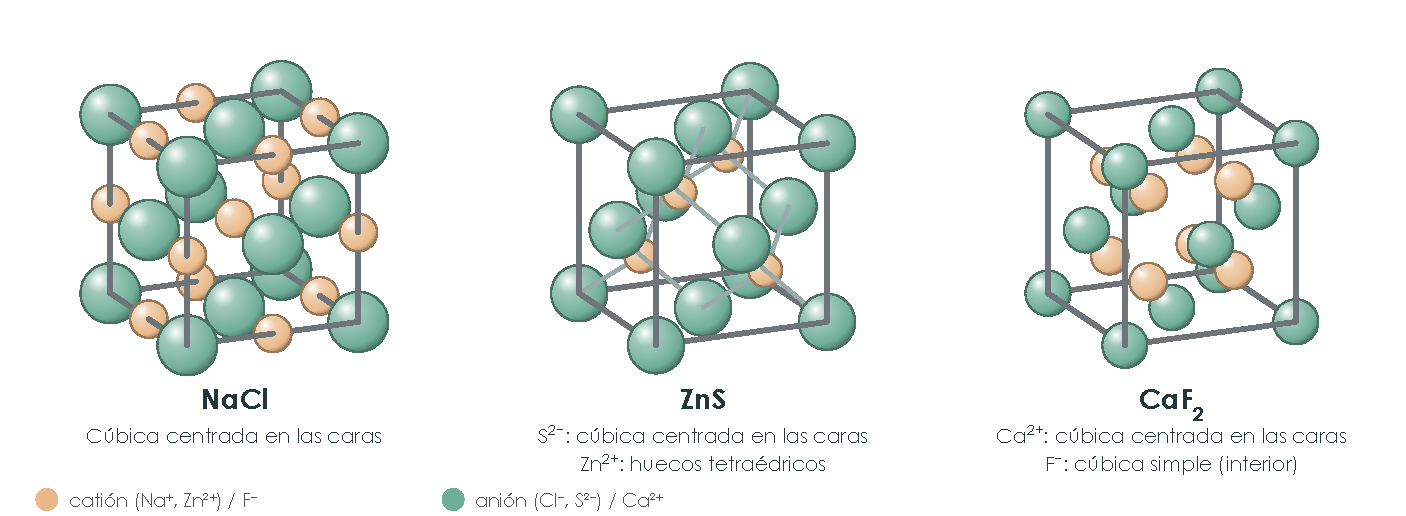
\includegraphics[width=0.95\linewidth]{FigurasSVG/UD3_Enlace_Quimico/pdf/UD3_01_redes_cristalinas.pdf}
    \caption{Redes cristalinas}
    \label{fig:redes_cristalinas}
\end{figure}

%    La descripción geométrica de estas agrupaciones de iones se hacen en función del:
%
%    \begin{enumerate}
%        \item Tipo de \blueremark{malla} u ordenación regular que adoptan.
%        \item \negrita{Número} ó \negrita{índice de coordinación}, siendo el número de iones de signo contrario que envuelven a un ion de signo contrario.
%    \end{enumerate}

% \begin{figure}[H]
%     \centering
%     \includegraphics[scale=0.45]{images/imagesUD3EnlaceQuimico/UD3_Teoria/redes_ionicas_tabla}
%     \caption{Tipos de principales redes iónicas y ejemplos de compuestos}
%     \label{fig:tipos_redes_ionicas}
% \end{figure}

\subsection{Teoría de Lewis sobre el enlace iónico}\label{subsec:teoria-de-lewis-sobre-el-enlace-ionico}

Según la teoría de Lewis, el enlace iónico es el proceso por el cual los átomos ganan, ceden o comparten electrones de las capas externas hasta conseguir la configuración de un gas noble.

Es importante introducir la \blueremark{estructura de Lewis} como aquella representación de los electrones del último nivel o capa de un átomo, ion o molécula, mediante puntos, círculos, cruces, rayas \dots

A continuación vemos la estructura de Lewis para algunos átomos neutros

\begin{figure}[H]
    \centering
    % [FIGURA ORIGINAL] \includegraphics[scale=0.45]{images/imagesUD3EnlaceQuimico/UD3_Teoria/lewis_atomos_neustros}
    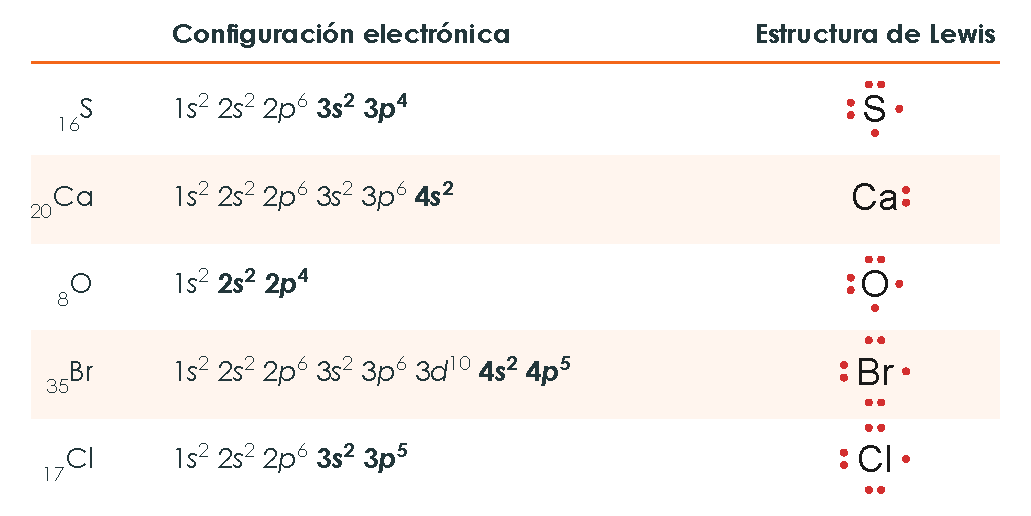
\includegraphics[width=0.8\linewidth]{FigurasSVG/UD3_Enlace_Quimico/pdf/UD3_02_lewis_atomos_neutros.pdf}
    \caption{Estructura de Lewis para átomos neutros}
    \label{fig:lewis_newtros}
\end{figure}

En el momento de la formación de un enlace iónico, se forman cationes y aniones, quedando, por tanto, su estructura de Lewis de la siguiente forma:

\begin{figure}[H]
    \centering
    % [FIGURA ORIGINAL] \includegraphics[scale=.45]{images/imagesUD3EnlaceQuimico/UD3_Teoria/lewis_iones}
    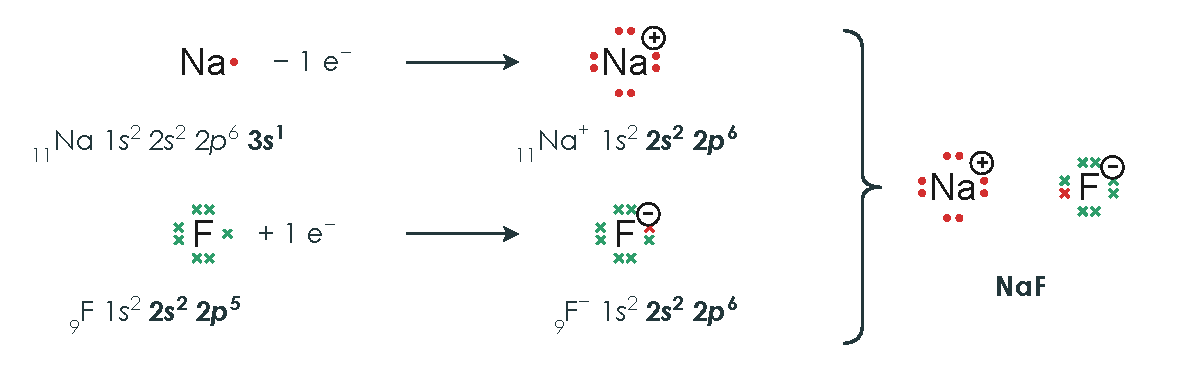
\includegraphics[width=0.85\linewidth]{FigurasSVG/UD3_Enlace_Quimico/pdf/UD3_03_lewis_iones.pdf}
    \caption{Estructura de Lewis para iones}
    \label{fig:lewis_iones}
\end{figure}

\subsection{Energía reticular \texorpdfstring{$\bm{U}$}{U}. Balance energético de la formación de un cristal iónico}\label{subsec:energia-reticular-texorpdfstring{$bm{u}$}{u}.-balance-energetico-de-la-formacion-de-un-cristal-ionico}

La \blueremark{energía reticular} (\(\bm{U}\)) la podemos definir de tres maneras diferentes:


    \begin{enumerate}[label=\letraminuscula]
            \item La energía necesaria para separar los iones que forman una red cristalina hasta una distancia infinita.
            En este caso la energía será positiva.
            \item \textbf{La energía que se desprende cuando dos iones en estado gaseoso se aproximan para formar un compuesto iónico. En este caso la energía será negativa.}
            \item La energía que hay que comunicar a un mol de un compuesto iónico para que sus iones se separen a una distancia que dejen de interaccionar.
            En este caso la energía será positiva.
    \end{enumerate}

La energía reticular nos determinará:
\begin{enumerate}[label=\letraminuscula]
        \item Estabilidad.
        \item Solubilidad.
        \item Dureza
\end{enumerate}

\subsection{Cálculo de la energía reticular}\label{subsec:calculo-de-la-energia-reticular}

La energía reticular la podemos calcular de manera experimental utilizando el ciclo de Born-Haber o de manera teórica usando la ecuación de Born-Landé.

\begin{enumerate}[label=\numberballmDarkTeal]
        \item \negrita{Ciclo de Born-Haber}.
        El ciclo de \textbf{Born-Haber} es un ciclo termodinámico en que se estudian, desde el punto de vista energético, todos los procesos que intervienen en la formación de un mol de un compuesto iónico a partir de las sustancias simples que lo integran cuando se encuentran en su estado termodinámico más estable.

        Como ejemplo veremos la formación del \ch{NaCl \sld{}} a partir de \ch{Na \sld{}} y \ch{Cl2 \gas{}} en su estado más estable.

        La energía del proceso se llama \textbf{entalpía de formación} del \ch{NaCl}, \(\Delta H_f\).

        \begin{equation*}
            \ch{Na \sld{} + 1/2 Cl2 \gas{} -> NaCl \sld{}} \qquad \qquad \Delta H_f = \energia[kjmol]{-411} \rightarrow \text{1 mol serán } \energia[kj]{-411}
        \end{equation*}

        Este paso global, lo podemos dividir en otros más sencillos o elementales:

        \begin{enumerate}[label=\numberballmDarkTeal]
            \item Sublimación del \ch{Na \sld{}} a \ch{Na \gas{}} para obtener los átomos de sodio aislados:
            \begin{equation*}
                \ch{Na \sld{}  -> Na \gas{}} \qquad  \Delta H_{sub} = \energia[kjmol]{107.3} \rightarrow \text{1 mol serán } \energia[kj]{107.3}
            \end{equation*}

            \item Disociación de las moléculas de \ch{Cl2 \gas{}} para obtener átomos de \ch{Cl} aislados, en este proceso tenemos que disociar \(\dfrac{1}{2}\) mol de moléculas de cloro:

            \begin{equation*}
                \ch{1/2 Cl2 \gas{}  -> Cl \gas{}} \qquad   \Delta H_{dis} = \energia[kjmol]{244} \rightarrow \dfrac{1}{2} \text{mol} \cdot 244 \unit{\kilo\joule\per\mole} =  \energia[kj]{122}
            \end{equation*}

            \item Ionización del \ch{Na \gas{}} a \ch{Na+ \gas{}} y para ello habrá que administrar la energía equivalente a la primera energía o potencial de ionización del sodio:

            \begin{equation*}
                \ch{Na \gas{}  -> Na+ \gas{}} \qquad   EI = \energia[kjmol]{495.8} \rightarrow  \text{1 mol serán }  \energia[kj]{495.8}
            \end{equation*}

            \item Ionización del \ch{Cl \gas{}} a \ch{Cl- \gas{}} en la que se desprenderá una energía equivalente a la primera afinidad electrónica del cloro:

            \begin{equation*}
                \ch{Cl \gas{}  -> Cl- \gas{}} \qquad   AE = \energia[kjmol]{-348.6} \rightarrow  \text{1 mol serán }  \energia[kj]{-348.6}
            \end{equation*}
            \item Energía reticular \(\bm{U}\), es la energía que se desprende al formar un mol de \ch{NaCl \sld{}} a partir de los iones constituyentes del estado gaseoso:

            \begin{equation*}
                \ch{Na+ \gas{} + Cl- \gas{} -> NaCl \sld{}} \qquad  \Delta U_r = \energia[kjmol]{-787} \rightarrow \text{1 mol serán } \energia[kj]{787}
            \end{equation*}

        \end{enumerate}

        Si aplicamos la Ley de Hess (el cambio de energía requerido en una reacción entre reactivos para dar productos es el mismo independientemente de que si la reacción se efectúe en un paso o en una serie de pasos):

        \begin{equation}
            \Delta H_{f} = \Delta H_{sub} + EI + \dfrac{1}{2} \Delta H_{dis} + AE + {\color {red} U_r}
        \end{equation}

        Si lo que queremos es obtener el valor de la energía reticular, basta con despejar y obtendremos:
        \begin{equation}
            {\color {red} U_r}
            = \Delta H_{f} - \Delta H_{sub} - EI - \dfrac{1}{2} \Delta H_{dis} - AE
        \end{equation}

        A continuación, se muestra un esquema del proceso:

        %   El \ch{NaCl} lo podemos formar a partir de sodio sólido y cloro molecular en estado gaseoso. Si mezclamos ambos reactivos no dará el \ch{NaCl} en estado sólido requiriéndose o desprendiéndose una determinada energía a la que llamamos entalpía de formación ($\Delta H_f$).

        \begin{figure}[H]
            \centering
            % [FIGURA ORIGINAL] \includegraphics[scale=1]{images/imagesUD3EnlaceQuimico/UD3_Teoria/cicloborhhabberNaCl}
            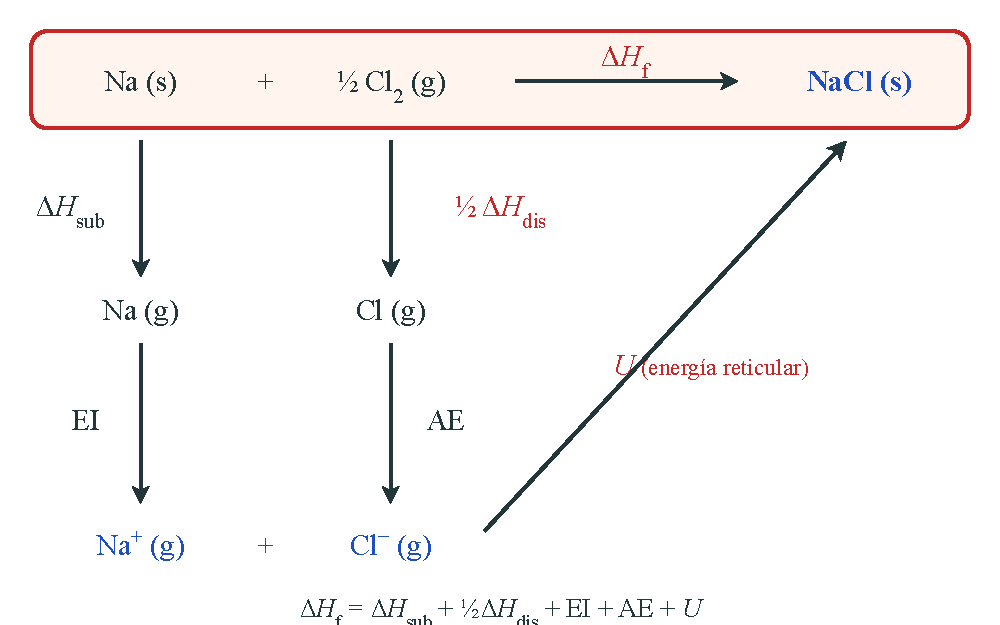
\includegraphics[width=0.75\linewidth]{FigurasSVG/UD3_Enlace_Quimico/pdf/UD3_04_ciclo_born_haber_NaCl.pdf}
            \caption{Ciclo de Born-Haber para el NaCl}
        \end{figure}

        \item \negrita{Ecuación de Born-Landé}
        \begin{equation}
            U_r = -\; N_A\ K\ \dfrac{Q_{\text{anión}}\ Q_{\text{catión}}}{d_0}\; A\ \left(1 - \dfrac{1}{n} \right)
            \label{eq:ecuacion_born_lande}
        \end{equation}

        Siendo:
        \begin{gather*}
            K = \text{Constante de Coulomb} = \dfrac{1}{4\pi\varepsilon_0} = \SI{9e9}{\N\square\metre\per\square \coulomb} (\text{en el vacío})\\
            Q_{\text{catión}} = \text{Carga del catión en Culombios}\\
            Q_{\text{anión}} = \text{Carga del anión en Culombios} \\
            A = \text{Constante de Madelung} \\
            d_0 = \text{distancia entre iones} = r_{\text{anión}} + r_{\text{catión}}\\
            n = \text{factor de Born}
        \end{gather*}
        A efectos prácticos, la \( Q_{\text{catión}} \) y \( Q_{\text{anión}} \) se le asignará el estado de oxidación de dicho ión.
%        Para calcular la carga tanto del anión como del catión sería: \(Q = | \text{carga de la especie} | \cdot | q_{\el} |\) siendo \(q_{\el} = \text{carga del electrón} = \SI{-1.6e-19}{\coulomb} \)
\end{enumerate}
El factor de Born es propio de cada par de iones.

La constante de Madelung, es una constante que depende del tipo de red cristalina que forma el compuesto iónico
%    ,siendo sus principales valores:
%
%    \begin{figure}[H]
%        \centering
%        \includegraphics[scale=0.45]{images/imagesUD3EnlaceQuimico/UD3_Teoria/valores_cte_madelung}
%        \caption{Valores de la constante de Madelung para algunas celdas iónicas}
%        \label{fig:constantedemadelungvalores}
%    \end{figure}

%    Para obtener el valor del factor de Born o compresibilidad que depende de la configuración electrónica de los iones, tenemos que conocer la siguiente tabla:
%
%
%    \begin{figure}[H]
%        \centering
%        \includegraphics[scale=.45]{images/imagesUD3EnlaceQuimico/UD3_Teoria/factor_de_born}
%        \caption{Factor de Born}
%        \label{fig:factor_born}
%    \end{figure}
%
%    Para conocer el valor del factor de Born para cada ión, tenemos que ver que configuración electronica adquiere cuando gana o pierde electrones. Luego determinamos que gas noble tiene la configuración electrónica adoptada y le asignamos a ese ión el valor que tenemos en la tabla anterior. Para conocer el valor total del compuesto iónico se hace la media aritmética de ambos factores de Born asignados a cada ión:
%
%
%    \begin{equation}
%        n_{\text{iónico}} = \dfrac{(n_{\text{anion}} + n_{\text{cation}})}{2}
%    \end{equation}
%
%    Por ejemplo, para determinar el el factor de Born par el \ch{NaCl}:
%
%    \begin{enumerate}[label=\numberballred]
%        \item \ch{Na}: \rojo{\elconf{11}} \ch{->} \ch{Na^+} quedando \azul{\elconf{10}} quedando la configuración de \negrita{\textcolor{mygreen}{\elementsymbol{10}}} quedando $n_{cation} = 7$.
%        \item \ch{Cl}: \rojo{\elconf{17}} \ch{->} \ch{Cl^-} quedando \azul{\elconf{18}} quedando la configuración de \negrita{\textcolor{mygreen}{\elementsymbol{18}}} quedando $n_{anion} = 9$.
%        \item Por lo tanto, el factor del Born para el \ch{NaCl} será:
%        \begin{equation*}
%            n_{NaCl} = \dfrac{7 + 9}{2} = 8
%        \end{equation*}
%    \end{enumerate}

\subsection{Propiedades de los compuestos iónicos}

\caja{Las propiedades de los compuestos iónicos, se derivan de su propia \blueremark{estructura} y de su naturaleza \blueremark{electrostática} del enlace entre los iones.}

Entre sus propiedades podemos destacar:

\begin{enumerate}[label=\numberballmDarkTeal]
        \item A temperatura ambiente, los compuestos iónicos son \negrita{\azul{sólidos cristalinos}}.
        \item Tienen elevados puntos de fusión y ebullición, debido a que hay que administrar mucha energía para destruir la estructura cristalina.
        \item A mayor ($\uparrow$) energía reticular mayor punto de fusión ($\uparrow$).
        \item No conducen la electricidad en estado sólido pero \negrita{\rojo{SI}} cuando están fundidos o en disolución, debido a la movilidad de sus iones.
        \item Son duros, a mayor energía reticular mayor dureza.
        \item Son frágiles y poco flexibles.
        \item Son solubles en disolventes polares, como el agua.
        Las moléculas de agua se van colocando alrededor de la estructura cristalina hasta que consigue romperla impidiendo que vuelvan a unirse.
        A la energía implicada en este proceso se le conoce como \azuln{energía de solvatación}
        \item Si la energía de solvatación es negativa y en valor absoluto superior a la \verden{energía reticular} la disolución será un proceso \verden{exotérmico} produciéndose así un aumento en la temperatura.
\end{enumerate}


\section{Enlace covalente}

En enlace covalente se da entre dos \azuln{no metales} o elementos del bloque \verden{p} de la tabla periódica.
La diferencia de electronegatividad no debe ser superior a 1.

El enlace covalente se dan normalmente entre elementos de los grupos 13 al 17 incluido el hidrógeno.

\subsection{Teoría de Lewis del enlace covalente}

\caja{Un \azuln{enlace covalente} se forma cuando dos átomos \azuln{comparten} un par de electrones. Por ejemplo:
    \begin{center}
        \lewis{H}{}{}{}{}{.}{}{}{} + \lewis{H}{}{.}{}{}{}{}{}{} \ch{->} \lewis{H}{}{}{}{}{}{}{}{}\hspace{-0.5em}---\hspace{-0.75em}\lewis{H}{}{}{}{}{}{}{}{}
    \end{center}
}

Lewis pensó que los gases nobles tenían la configuración más estable posible, ya que no formaban compuestos y, por tanto, los demás elementos hacían todo lo posible por adquirir una configuración de gas noble que le diera estabilidad.
Al tener los gases nobles ocho electrones en su última capa (a excepción del \ch{He}) se le llamó  \azuln{regla del octeto}.
Esto se demuestra con la formación de \ch{F2}.

%    \begin{figure}[H]
%        \centering
%        \includegraphics[scale=1]{images/imagesUD3EnlaceQuimico/UD3_Teoria/formacionf2_lewis}
%        \caption{Formación de \ch{F2}. Estructura de Lewis}
%        \label{fig:f2_covalente}
%    \end{figure}

\begin{figure}[H]
    \centering
    % [FIGURA ORIGINAL] \includegraphics[scale=0.5]{images/imagesUD3EnlaceQuimico/UD3_Teoria/lewis_F2}
    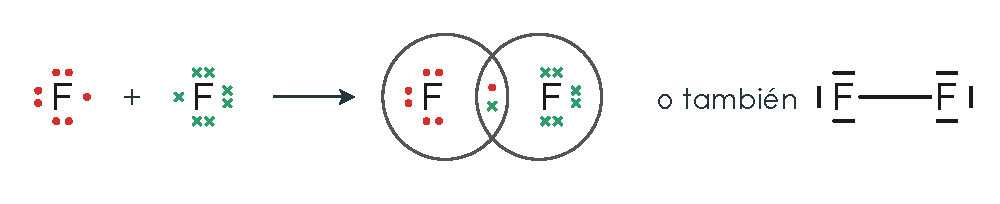
\includegraphics[width=0.7\linewidth]{FigurasSVG/UD3_Enlace_Quimico/pdf/UD3_05_formacion_F2_lewis.pdf}
    \caption{Formación de \ch{F2}. Estructura de Lewis}
    \label{fig:f2_covalente}
\end{figure}
Algo similar tendremos para el agua, amoniaco o nitrógeno
\begin{figure}[H]
    \centering
    % [FIGURA ORIGINAL] \includegraphics[scale=0.5]{images/imagesUD3EnlaceQuimico/UD3_Teoria/lewis_agua_amoniaco_nitrogeno}
    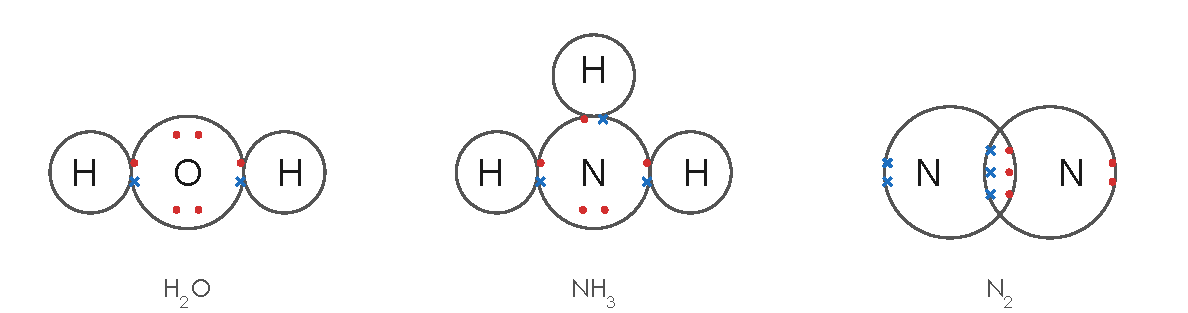
\includegraphics[width=0.85\linewidth]{FigurasSVG/UD3_Enlace_Quimico/pdf/UD3_06_lewis_agua_amoniaco_nitrogeno.pdf}
    \caption{Formación agua, amoniaco y nitrógeno}
    \label{fig:agua_amoniaco_nitrogeno}
\end{figure}

Algunas veces los átomos pueden alcanzar su octeto compartiendo dos o tres pares de electrones para formar así un doble o un triple enlace (ver Figura~\ref{fig:estructuras_lewis} más adelante)

Llamamos \azuln{orden de enlace} al número de pares de electrones compartidos en una molécula.

\subsection{Reglas para escribir estructuras de Lewis}
Para escribir correctamente las estructuras de Lewis podemos seguir los siguientes pasos (tomaremos como ejemplo la formación de \ch{F2}):

\begin{enumerate}[label=\numberballmDarkTeal]
        \item Sumar los electrones de valencia de los átomos $7 + 7 = 14$ \elec.
        Los llamaremos electrones de valencia (EV).

        \item Calculamos los pares de electrones de valencia (PEV) según $\dfrac{\text{electrones de valencia}}{2}$.Para el \ch{F2} tendremos $\dfrac{14}{2} = 7$.

        \item Contar los electrones que necesitaríamos para que todos los átomos completaran la configuración de gas noble, es decir completaran el octeto a excepción del hidrógeno que le contabilizaríamos 2 electrones. $8 \times 2 = 16$ \elec.
        Los llamaremos electrones del octeto.

        \item Calculamos los pares de electrones enlazantes (PE) según:
        \begin{equation}
            PE = \dfrac{\text{electrones del octeto} - \text{electrones de valencia}}{2}
        \end{equation}
        En el caso del \ch{F2} tendremos que: $\dfrac{16 - 14}{2} = 1$
        \item Ahora calculamos los pares de electrones no enlazantes (PEN) según:
        \begin{equation}
            PEN = PEV - PE
        \end{equation}
        En el caso del \ch{F2} tendremos que: $PEN = 7 - 1 = 6$
        \item Situamos ahora los átomos poniendo el átomo central aquel que sea menos electronegativo a excepción del hidrógeno que nunca se pondrá en el centro.

        \item Ahora vamos colocando los pares de electrones enlazantes (son los que enlazan a otros átomos) y no enlazantes (se sitúan alrededor de cada átomo) de manera que se vayan completando el octeto en todos los átomos
        \begin{figure}[H]
            \centering
            % [FIGURA ORIGINAL] \includegraphics[scale=1]{images/imagesUD3EnlaceQuimico/UD3_Teoria/F2_lewis}
            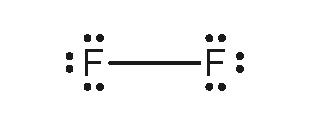
\includegraphics[width=0.22\linewidth]{FigurasSVG/UD3_Enlace_Quimico/pdf/UD3_07_F2_lewis.pdf}
            \caption{Estructura de Lewis para el \ch{F2}}
            \label{fig:fluor_lewis}
        \end{figure}
\end{enumerate}
A continuación se muestran más ejemplos de estructuras de Lewis:
\begin{figure}[H]
    \centering
    % [FIGURA ORIGINAL] \includegraphics[scale=1]{images/imagesUD3EnlaceQuimico/UD3_Teoria/lewis_varios}
    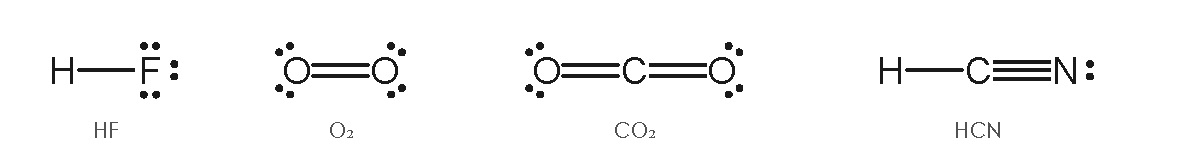
\includegraphics[width=0.8\linewidth]{FigurasSVG/UD3_Enlace_Quimico/pdf/UD3_08_lewis_varios.pdf}
    \caption{Estructuras de Lewis}
    \label{fig:estructuras_lewis}
\end{figure}

\subsection{Excepciones a la regla del octeto}

Podemos tener dos posibles casos, octetos incompletos y octetos ampliados.

\begin{enumerate}[label=\numberballmDarkTeal]
        \item \textbf{Octetos incompletos}: existen átomos que puede formar compuestos sin llegar a completar el octeto, son el caso del \blueremark{boro} y \blueremark{aluminio}.
        En estos casos, llegaran a tener 6 electrones en lugar de 8.
        \begin{figure}[H]
            \centering
            % [FIGURA ORIGINAL] \includegraphics[scale=1]{images/imagesUD3EnlaceQuimico/UD3_Teoria/octeto_incomleto}
            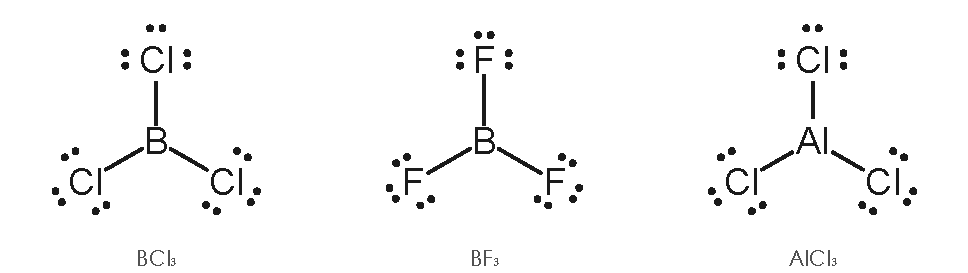
\includegraphics[width=0.7\linewidth]{FigurasSVG/UD3_Enlace_Quimico/pdf/UD3_09_octeto_incompleto.pdf}
            \caption{\ch{BCl3}, \ch{BF3} y \ch{AlCl3}}
            \label{fig:octetoincompleto}
        \end{figure}
        \item \textbf{Octeto ampliado}: a partir del tercer periodo, los elementos presentan orbitales $d$ vacíos y por lo tanto los átomos pueden ampliar su capa de valencia a 10, 12 o más electrones.
        Esto nos permite formar más enlaces de los previstos según la regla de Lewis, estos casos los encontramos principalmente en el \blueremark{azufre} y en el \blueremark{fósforo}
        \begin{figure}[H]
            \centering
            % [FIGURA ORIGINAL] \includegraphics[scale=1]{images/imagesUD3EnlaceQuimico/UD3_Teoria/Lewis_Octeto_Ampliado}
            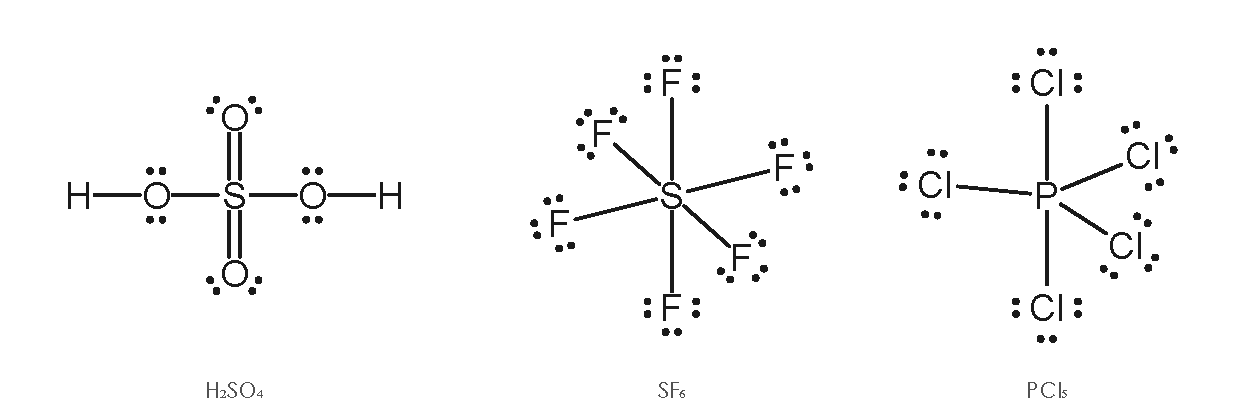
\includegraphics[width=0.8\linewidth]{FigurasSVG/UD3_Enlace_Quimico/pdf/UD3_10_octeto_ampliado.pdf}
            \caption{\ch{H2SO4}, \ch{SF6} y \ch{PCl5}}
            \label{fig:octetoampliado}
        \end{figure}
        \item \textbf{Moléculas con número impar de electrones}: se da cuando la suma de los electrones de valencia suman un número impar.
        En estos casos al menos uno de los átomos no conseguirá completar el octeto.
        Un ejemplo sería el \ch{NO}
        \begin{figure}[H]
            \centering
            % [FIGURA ORIGINAL] \includegraphics[scale=1]{images/imagesUD3EnlaceQuimico/UD3_Teoria/NO}
            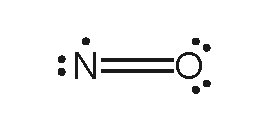
\includegraphics[width=0.18\linewidth]{FigurasSVG/UD3_Enlace_Quimico/pdf/UD3_11_NO_lewis.pdf}
            \caption{\ch{NO}}
            \label{fig:numeroimparelectrones}
        \end{figure}
\end{enumerate}

\marcador{Escribir las siguientes estructuras de Lewis}: Escribir la estructura de lewis para \ch{H2SO3}, \ch{HNO3}, \ch{CH4}, \ch{CCl4}

\subsection{Resonancia}\label{subsec:resonancia}

En algunas ocasiones, podemos escribir más de una estructura de Lewis para un mismo compuesto.
Al conjunto de estas estructuras de Lewis se les denomina \negrita{estructuras resonantes}.

\begin{figure}[H]
    \centering
    % [FIGURA ORIGINAL] \includegraphics[scale=1]{images/imagesUD3EnlaceQuimico/UD3_Teoria/estructuras_resonantes_NO3}
    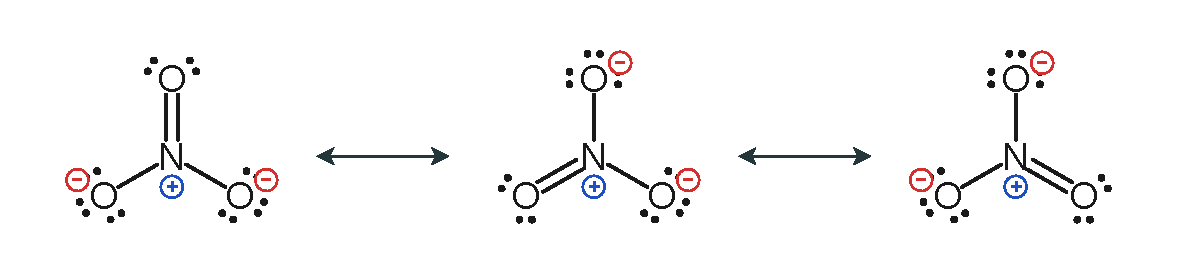
\includegraphics[width=0.85\linewidth]{FigurasSVG/UD3_Enlace_Quimico/pdf/UD3_12_resonancia_NO3.pdf}
    \caption{Estructuras resonantes de ión nitrato \ch{NO3-}}
    %\label{fig:}
\end{figure}

Aunque podamos escribir varias estructuras resonantes siempre habrá alguna de ellas que contribuya más, es decir, tendremos una serie de posibles estructuras, pero siempre habrá alguna mayoritaria.
%    y para ello podemos seguir las siguientes reglas:
%    \begin{enumerate}[label=\numberballmDarkTeal]
%        \item Las estructuras resonantes sólo suponen movimiento de electrones desde posiciones adyacentes (nunca de átomos).
%        El movimiento de electrones se representan con flechas.
%        \item Las estructuras resonantes en las que los átomos del segundo periodo poseen octetos completos son más importantes que las que tienen octetos incompletos.
%        \item Las estructuras más importantes son aquellas que supongan la \negrita{mínima separación de cargas}.
%        Se debe intentar no tener cargas en los átomos.
%        \item En los casos en que una estructura de Lewis con octetes completos no puede representarse sin separación de cargas, la estructura más importante será aquella en la que la carga negativa se sitúa sobre el átomo más electronegativo y la carga positiva en el átomo menos electronegativo (más electropositivo).
%    \end{enumerate}
Las estructuras resonantes sólo suponen movimiento de electrones desde posiciones adyacentes (nunca de átomos).
El movimiento de electrones se representan con flechas.

\subsection{Conceptos importantes del enlace covalente}

Existen una serie de definiciones, propiedades o parámetros relevantes del enlace covalente que las podemos resumir de la siguiente manera:

\begin{enumerate}[label=\numberballmDarkTeal]
        \item \negrita{Longitud de enlace}: distancia entre los átomos enlazados.
        \item \negrita{Ángulo de enlace}: solo tiene sentido en moléculas de más 3 de átomos y será el ángulo que forman dos enlaces compartiendo un átomo común.
        \item \negrita{Entalpía de enlace}: es la energía que se debe suministrar o se libera cuando se rompe un enlace, un enlace sencillo tendrá menos energía que un enlace doble y este a su vez que un enlace triple.
        \begin{figure}[H]
            \centering
            % [FIGURA ORIGINAL] \includegraphics[scale=0.45]{images/imagesUD3EnlaceQuimico/UD3_Teoria/entalpiasyenlacespromedio}
            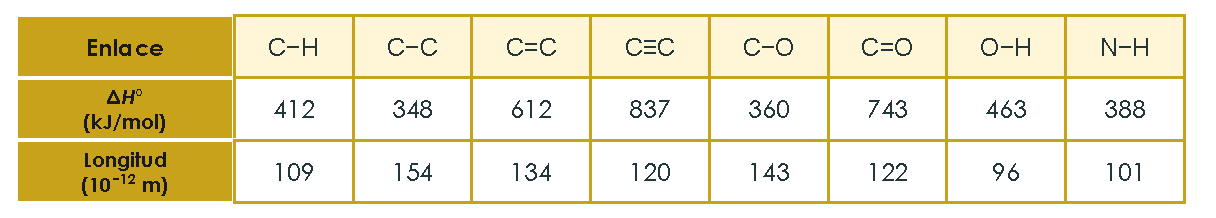
\includegraphics[width=0.95\linewidth]{FigurasSVG/UD3_Enlace_Quimico/pdf/UD3_13_entalpias_longitudes_enlace.pdf}
            \caption{Entalpías promedio y longitudes de enlace promedio.}
            \label{fig:entalpiasyenlaces}
        \end{figure}
        \item \negsubro{Polaridad de enlaces y moléculas}: se produce cuando existen electronegatividades diferentes entre dos átomos que forman un enlace introduciendo así una carga parcial positiva ($\delta +$)  en el elemento menos electronegativo o negativa ($\delta -$) en el elemento más electronegativo.

        Para cuantificar la polaridad de un enlace utilizaremos el \azuln{momento dipolar, $\mu$} que equivale al producto entre la carga neta ($q$) y la distancia internuclear ($r$) según la expresión.
        \begin{equation}
            \tcboxmath[opteqA]{\mu = q\; r}
        \end{equation}
        El momento dipolar es un vector orientado desde el polo positivo (átomo menos electronegativo) hacia el polo negativo (átomo más electronegativo).
        La unidad en el S.I es el \azuln{\si{\coulomb\metre}}.
        Hay que tener en cuenta que el momento dipolar nos da una medida de la polarización de dicho enlace y no hay que confundirlo con la \azuln{polaridad de una molécula}.
        Para saber si una molécula es polar, es decir presenta un momento dipolar distinto de cero, tenemos que sumar todos los momentos dipolares de todos los enlaces de la molécula y si el momento dipolar resultante es distinto de cero entonces diremos que la molécula es \azuln{polar} y si el resultado del momento dipolar resultante es cero, entonces decimos que la molécula es \azuln{apolar}
        \begin{figure}[H]
            \centering
            % [FIGURA ORIGINAL] \includegraphics[scale=1]{images/imagesUD3EnlaceQuimico/UD3_Teoria/polaridad_nuevo}
            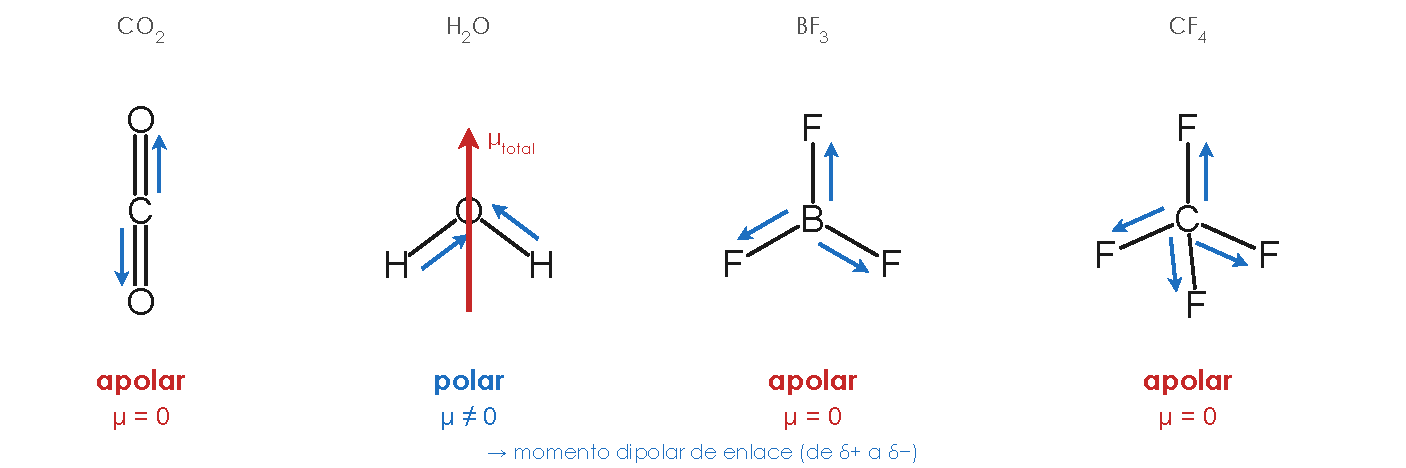
\includegraphics[width=0.9\linewidth]{FigurasSVG/UD3_Enlace_Quimico/pdf/UD3_14_polaridad_moleculas.pdf}
            \caption{Moléculas polares y apolares}
            \label{fig:moleculaspolaresyapolares}
        \end{figure}

        Los \textbf{pares de electrones no enlazantes} también contribuyen al momento dipolar de las moléculas, pues estos pares electrónicos tienden a concentrar la carga electrónica sobre el átomo al que pertenecen.
        Este efecto justifica por qué la molécula de \ch{NH3} tiene un momento dipolar mayor que \ch{NF3}

        Por norma general (aunque no siempre, habrá que estudiar cada caso en concreto) si sobre un átomo central, los átomos a los que está unido no son todos iguales, la molécula suele ser \textbf{polar} mientras que si los átomos a los que se unen dependerá de la geometría la molécula y el número de pares de electrones enlazantes.
        En la siguiente tabla, se muestran el tipo de polaridad que tendría una molécula si todos los átomos a los que se une el átomo central son iguales.

        \begin{longtblr}[
            caption = {Polaridad de una molécula según su geometría cuando los átomos unidos al átomo central son iguales},
        ]{
            colspec = {|Q[c,m]|Q[c,m]|},
            rowhead = 1,
            row{1} = {bg=mybluecolour, fg = white, font=\sffamily},
        %vlines = {1}{white},
        }
            \hline
            Geometría                                   & Polaridad \\
            \hline
            Lineal                                      & Apolar    \\
            \hline
            Trigonal plana (triangular)                 & Apolar    \\
            \hline
            Angular                                     & Polar     \\
            \hline
            Tetraédrica                                 & Apolar    \\
            \hline
            Pirámide trigonal                           & Polar     \\
            \hline
            Bipirámide trigonal (bipirámide triangular) & Polar     \\
            \hline
            Tetraédrica distorsionada                   & Polar     \\
            \hline
            En forma de T                               & Polar     \\
            \hline
            Octaédrica                                  & Apolar    \\
            \hline
            Pirámide cuadrada                           & Polar     \\
            \hline
            Plano cuadrada                              & Apolar    \\
            \hline
        \end{longtblr}



        \item \negsubro{Polarizables y polarizantes}: podemos decir que un átomo o ion es \azuln{polarizable} cuando su nube electrónica experimenta fácilmente grandes deformaciones de modo que puede inducirse en un extremo del átomo más carga electrónica que en el otro extremo y, por lo tanto, aparición de un dipolo (molécula con un $\delta +$ y $\delta -$). En general, los iones grandes como el \ch{I-} son altamente polarizables.
        Un átomo o ion es \azuln{polarizante} cuando puede producir esas grandes deformaciones en las nubes electrónicas.
        Son buenos polarizantes los cationes pequeños y elevadas cargas.
\end{enumerate}

%    \begin{enumerate}[label=\numberballmDarkBrown]
%        \item \negsubro{Radicales}: es un fragmento de molécula con algún electrón desapareado, provienen fundamentalmente de la ruptura homolítica de enlaces en el cual el par de electrones que formaban el enlace se reparte uno para cada átomo. Como ejemplos vemos el radical metilo y el radical hidroxilo.
%        \begin{figure}[H]
%            \centering
%            \includegraphics[scale=1]{images/imagesUD3EnlaceQuimico/UD3_Teoria/radicales.eps}
%            \caption{Radicales metilo e hidroxilo}
%            \label{fig:radicalmetilohidroxilo}
%        \end{figure}
%        \item \negrita{\coloruline{red}{Parámetros del enlace covalente}}
%        \begin{enumerate}
%            \item \negrita{Longitud de enlace}: distancia entre los átomos enlazados.
%            \item \negrita{Ángulo de enlace}: solo tiene sentido en moléculas de más 3 de átomos y será el ángulo que forman dos enlaces compartiendo un átomo común.
%            \item \negrita{Entalpía de enlace}: es la energía que se debe suministrar o se libera cuando se rompe un enlace, un enlace sencillo tendrá menos energía que un enlace doble y este a su vez que un enlace triple.
%            \begin{figure}[H]
%                \centering
%                \includegraphics[scale=0.45]{images/imagesUD3EnlaceQuimico/UD3_Teoria/entalpiasyenlacespromedio.png}
%                \caption{Entalpías promedio y longitudes de enlace promedio.}
%                \label{fig:entalpiasyenlaces}
%            \end{figure}
%        \end{enumerate}
%        \item \negsubro{Polaridad de enlaces y moléculas}: se produce cuando existen electronegatividades diferentes entre dos átomos que forman un enlace introduciendo así una carga parcial positiva ($\delta +$) o negativa ($\delta -$) en cada átomo.
%
%        Para cuantificar la polaridad de un enlace utilizaremos el \azuln{momento dipolar, $\mu$} que equivale al producto entre la carga neta ($q$) y la distancia internuclear ($r$) según la expresión.
%        \begin{equation}
%            \tcboxmath[opteqA]{\mu = q\; r}
%        \end{equation}
%        El momento dipolar es un vector orientado desde el polo positivo (átomo menos electronegativo) hacia el polo negativo (átomo más electronegativo). La unidad en el S.I es el \azuln{\si{\coulomb\metre}}.
%        Hay que tener en cuenta que el momento dipolar nos da una medida de la polarización de dicho enlace y no hay que confundirlo con la \azuln{polaridad de una molécula}. Para saber si una molécula es polar, es decir presenta un momento dipolar distinto de cero, tenemos que sumar todos los momentos dipolares de todos los enlaces de la molécula y si el momento dipolar resultante es distinto de cero entonces diremos que la molécula es \azuln{polar} y si el resultado del momento dipolar resultante es cero, entonces decimos que la molécula es \azuln{apolar}
%        \begin{figure}[H]
%            \centering
%            \includegraphics[scale=1]{images/imagesUD3EnlaceQuimico/UD3_Teoria/polaridad.eps}
%            \caption{Moléculas polares y apolares}
%            \label{fig:moleculaspolaresyapolares}
%        \end{figure}
%
%        Los \textbf{pares de electrones no enlazantes} también contribuyen al momento dipolar de las moléculas, pues estos pares electrónicos tienden a concentrar la carga electrónica sobre el átomo al que pertenecen. Este efecto justifica por qué la molécula de \ch{NH3} tiene un momento dipolar mayor que el \ch{NF3}
%
%        Por norma general (aunque no siempre, habrá que estudiar cada caso en concreto) si sobre un átomo central, los átomos a los que está unido no son todos iguales, la molécula suele ser \textbf{polar} mientras que si los átomos a los que se unen dependerá de la geometría la molécula y el número de pares de electrones enlazantes. En la siguiente tabla, se muestran el tipo de polaridad que tendría una molécula si todos los átomos a los que se une el átomo central son iguales.
%
%        \begin{longtblr}[
%            caption = {Polaridad de una molécula según su geometría cuando los átomos unidos al átomo central son iguales},
%        ]{
%            colspec = {|Q[c,m]|Q[c,m]|},
%            rowhead = 1,
%            row{1} = {bg=mybluecolour, fg = white, font=\sffamily},
%            vlines = {1}{white},
%        }
%            \hline
%            Geometría                                                                                                                                & Polaridad \\
%            \hline
%            {\includegraphics[scale=.5]{images/imagesUD3EnlaceQuimico/UD3_Teoria/lineal.png}  Lineal}                                                  & Apolar    \\
%            \hline
%            {\includegraphics[scale=0.5]{images/imagesUD3EnlaceQuimico/UD3_Teoria/trigonal.png}  Trigonal plana (triangular)}                          & Apolar     \\
%            \hline
%            {\includegraphics[scale=0.5]{images/imagesUD3EnlaceQuimico/UD3_Teoria/angular.png} Angular}                                                & Polar     \\
%            \hline
%            {\includegraphics[scale=0.5]{images/imagesUD3EnlaceQuimico/UD3_Teoria/tetraedrica.png} Tetraédrica }                                       & Apolar    \\
%            \hline
%            {\includegraphics[scale=.5]{images/imagesUD3EnlaceQuimico/UD3_Teoria/piramidetrigonal.png}  Pirámide trigonal}                             & Polar     \\
%            \hline
%            {\includegraphics[scale=.5]{images/imagesUD3EnlaceQuimico/UD3_Teoria/bipiramidetrigonal.png}  Bipirámide trigonal (bipirámide triangular)} & Polar     \\
%            \hline
%            {\includegraphics[scale=.5]{images/imagesUD3EnlaceQuimico/UD3_Teoria/tetraedricadistorsionada.png} Tetraédrica distorsionada }             & Polar     \\
%            \hline
%            {\includegraphics[scale=.5]{images/imagesUD3EnlaceQuimico/UD3_Teoria/enformadeT} En forma de T}                                        & Polar     \\
%            \hline
%            {\includegraphics[scale=.5]{images/imagesUD3EnlaceQuimico/UD3_Teoria/octaedrica.png}  Octaédrica}                                          & Apolar    \\
%            \hline
%            {\includegraphics[scale=.5]{images/imagesUD3EnlaceQuimico/UD3_Teoria/piramidalcuadrada.png}  Pirámide cuadrada}                            & Polar     \\
%            \hline
%            {\includegraphics[scale=.5]{images/imagesUD3EnlaceQuimico/UD3_Teoria/planacuadrada.png}  Plano cuadrada}                                   & Apolar    \\
%            \hline
%        \end{longtblr}
%
%
%
%        \item \negsubro{Polarizables y polarizantes}: podemos decir que un átomo o ion es \azuln{polarizable} cuando su nube electrónica experimenta fácilmente grandes deformaciones de modo que puede inducirse en un extremo del átomo más carga electrónica que en el otro extremo y por lo tanto aparición de un dipolo (molécula con un $\delta +$ y $\delta -$). En general, los iones grandes como el \ch{I-} son altamente polarizables.
%        Un átomo o ion es \azuln{polarizante} cuando puede producir esas grandes deformaciones en las nubes electrónicas.
%        Son buenos polarizantes los cationes pequeños y elevadas cargas.
%    \end{enumerate}

\subsection{Enlace covalente dativo o coordinado}

\caja{En un \azuln{enlace covalente dativo} es aquel en el que los dos electrones son donados por un átomo. Para que el enlace se produzca uno de los átomos tiene que disponer de un par electrones libre y el otro debe disponer de un orbital libre para aceptarlos}

El enlace covalente dativo se representa mediante una flecha que va desde el átomo donador al átomo aceptor ($A \rightarrow B$)

%    \begin{figure}[H]
%        \centering
%        \includegraphics[scale=1]{images/imagesUD3EnlaceQuimico/UD3_Teoria/dativoamonio}
%        \caption{Enlace covalente dativo}
%        \label{fig:enlacecovalentedativo}
%    \end{figure}


% \begin{figure}[H]
%     \centering
%     \includegraphics[scale=1]{covalente dativo.png}
%     \caption{Enlace covalente dativo}
%     \label{fig:enlacecovalentedativo}
% \end{figure}

Ejemplos de la formación del enlace covalente dativo,lo podemos encontrar en:
\begin{enumerate}[label=\numberballmDarkBrown]
        \item \negsubro{Ion Amonio (\ch{NH4^+})}:
        \begin{figure}[H]
            \centering
            % [FIGURA ORIGINAL] \includegraphics[scale=.5]{images/imagesUD3EnlaceQuimico/UD3_Teoria/dativoamonio}
            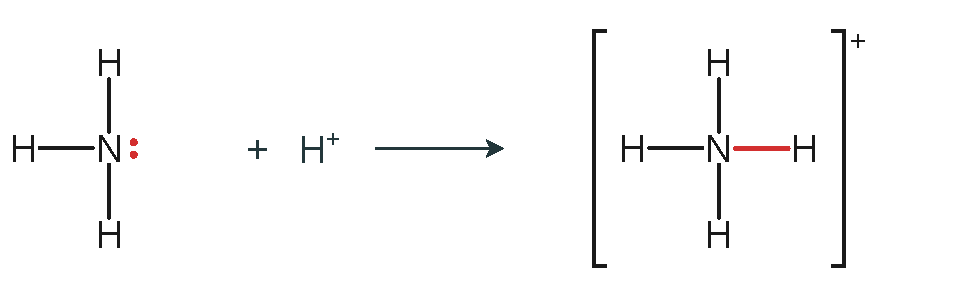
\includegraphics[width=0.7\linewidth]{FigurasSVG/UD3_Enlace_Quimico/pdf/UD3_15_dativo_amonio.pdf}
            \caption{Enlace dativo en el ion amonio}
            \label{fig:dativoamonio}
        \end{figure}
        \item \negsubro{Ion Oxonio (\ch{H3O^+})}:
        \begin{figure}[H]
            \centering
            % [FIGURA ORIGINAL] \includegraphics[scale=.5]{images/imagesUD3EnlaceQuimico/UD3_Teoria/dativooxonio}
            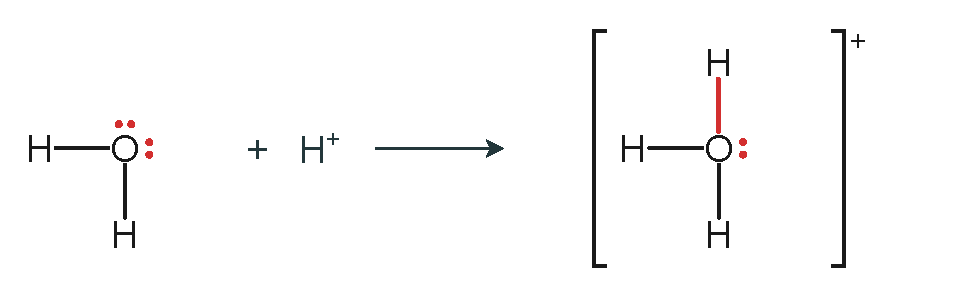
\includegraphics[width=0.7\linewidth]{FigurasSVG/UD3_Enlace_Quimico/pdf/UD3_16_dativo_oxonio.pdf}
            \caption{Enlace dativo en el ion oxonio}
            \label{fig:dativoxonio}
        \end{figure}
\end{enumerate}

\subsection{Teoría de la repulsión entre pares de electrones de valencia (TRPECV)}\label{subsec:teoria-de-la-repulsion-entre-pares-de-electrones-de-valencia-(trpecv)}
\caja{Todos los pares electrónicos (enlazantes y no enlazantes) de la capa de valencia de los átomos que forman los enlaces covalentes se sitúan lo más alejado posible unos de los otros, de manera que las repulsiones sean las mínimas. Esta teoría explica la \rojon{geometría} de las sustancias covalentes}

El factor determinante de la geometría de la molécula es el número de pares de electrones de valencia, tanto enlazantes como no enlazantes que tenemos alrededor del átomo central.
En la siguiente figura, podemos ver como las repulsiones electrónicas entre los pares de electrones no enlazantes y los enlazantes-no enlazantes en la molécula de agua hacen que el ángulo teórico de \ang{180} se cierre quedando finalmente en un ángulo real de \ang{104.5}.
Esta geometría es angular y no lineal.
\begin{figure}[H]
    \centering
    % [FIGURA ORIGINAL] \includegraphics[scale=0.5]{images/imagesUD3EnlaceQuimico/UD3_Teoria/respulsiones electrónicas}
    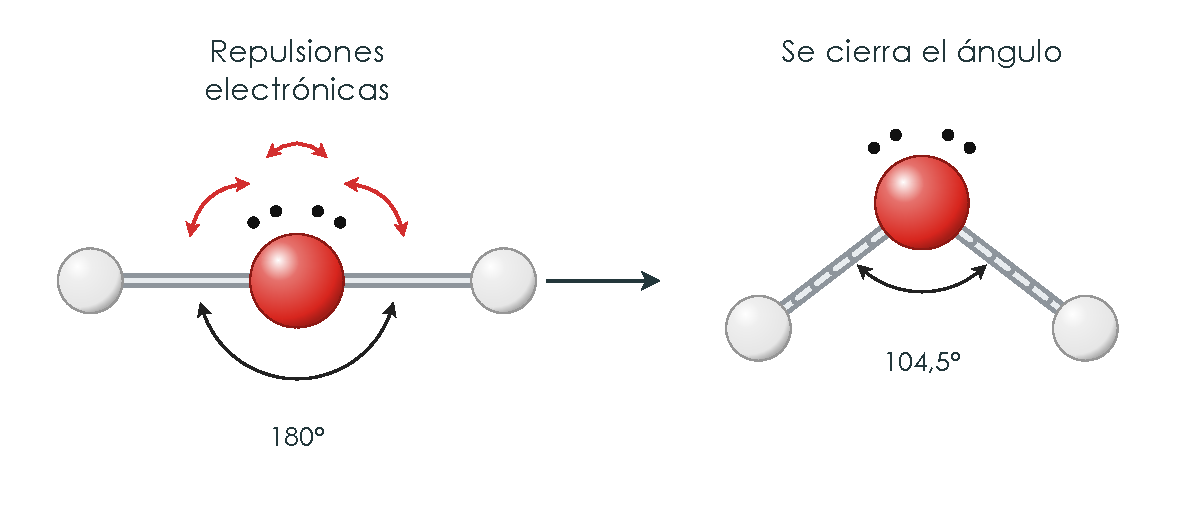
\includegraphics[width=0.75\linewidth]{FigurasSVG/UD3_Enlace_Quimico/pdf/UD3_17_repulsiones_electronicas.pdf}
    \caption{Repulsiones electrónicas en la molécula de agua.}
    \label{fig:repulsionesagua}
\end{figure}

%    {\large{} \textbf{\textcolor{blue}{Postulados del modelo TRPECV}}}

% Los postulados básicos de la TRPECV son:
%    \begin{enumerate}[label=\numberballmDarkBrown]
%        \item El factor determinante de la geometría de la molécula es el número de pares de electrones de valencia, tanto enlazantes como no enlazantes que tenemos alrededor del átomo central.
%        \item Se cuenta el número de zonas de alta densidad electrónica entorno al átomo central sin distinguir entre enlaces y pares de electrones solitarios.
%        \item Se representan gráficamente las orientaciones espaciales de mínima repulsión (los pares no compartidos ocupan más espacio que los compartidos).
%        \item Se colocan los átomos que rodean al átomo central en los extremos de las nubes electrónicas.
%        \item Se obtiene la geometría molecular a partir de la disposición espacial de los núcleos de los átomos presentes (no de las nubes electrónicas). La geometría real se predice teniendo en cuenta las distorsiones angulares generadas por los diferentes pares de enlace o pares solitarios.
%
%        En la siguiente figura, podemos ver como las repulsiones electrónicas entre los pares de electrones no enlazantes y los enlazantes-no enlazantes en la molécula de agua hacen que el ángulo teórico de \ang{180} se cierre quedando finalmente en un ángulo real de \ang{104.5}. Esta geometría es angular y no lineal.
%        \begin{figure}[H]
%            \centering
%            \includegraphics[scale=0.5]{images/imagesUD3EnlaceQuimico/UD3_Teoria/respulsiones electrónicas.png}
%            \caption{Repulsiones electrónicas en la molécula de agua.}
%            \label{fig:repulsionesagua}
%        \end{figure}
%    \end{enumerate}

\subsubsection[Geometría sin pares de electrones no enlazantes]{Geometría de las moléculas cuyo átomo central carece de pares de electrones solitarios o no enlazantes}

Vamos a suponer que la molécula a estudiar tiene un átomo central (A) y unido a el, otro átomo o conjunto de átomos (pueden ser iguales o diferentes) que los nombraremos como B.
Al no tener pares de electrones no enlazantes la geometría general de la molécula la podemos escribir como \ch{AB_n} donde $n$ puede variar entre 2 y 6.
Siendo \( n \) el número de átomo unidos al átomo central que pueden ser todos iguales o diferentes, por ejemplo la molécula \ch{H2O} sería del tipo \( AB_2 \) (el \ch{O} es el átomo central \( A \) mientras que los hidrógenos serán los átomos \( B \) ), la molécula \ch{CH4} (el \ch{C} es el átomo central \( A \) y los hidrógenos los átomos \( B \)) sería del tipo \( AB_4 \) y la molécula \ch{BF2Cl} (el átomo central \( A  \) sería el boro mientras que que los átomos \( B \) serían en este caso el \ch{F} y el \ch{Cl}) sería del tipo \( AB_3 \)

\begin{enumerate}[label=\numberballmDarkTeal]
        \item \negrita{Molécula del tipo \ch{AB2}}: son moléculas con geometría \azuln{lineal} y tienen un ángulo de \rojon{\ang{180}}.
        Ejemplos: \ch{CO2}, \ch{BeH2}.
        \begin{figure}[H]
            \centering
            % [FIGURA ORIGINAL] \includegraphics[scale=0.5]{images/imagesUD3EnlaceQuimico/UD3_Teoria/GEOMETriaCO2}
            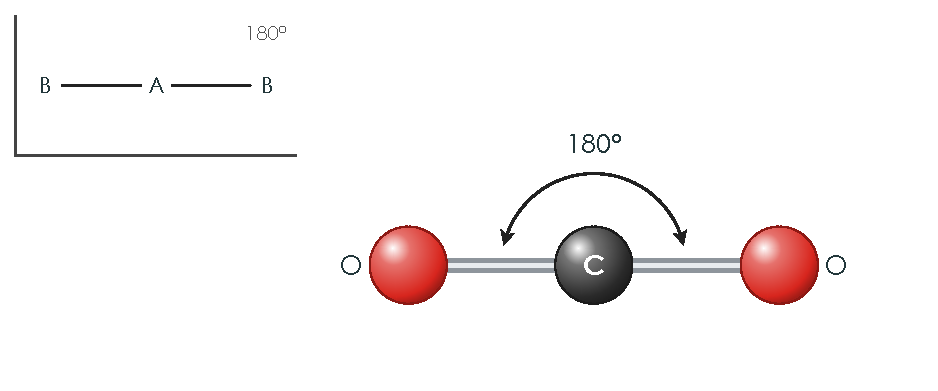
\includegraphics[width=0.6\linewidth]{FigurasSVG/UD3_Enlace_Quimico/pdf/UD3_18_geometria_CO2.pdf}
            \caption{Geometría de la molécula \ch{CO2}}
            \label{fig:GeometriadelamoleculaCO2}
        \end{figure}
        \item \negrita{Molécula del tipo \ch{AB3}}: son moléculas con geometría \azuln{trigonal plana}, con ángulos de enlace de \rojon{\ang{120}}. Ejemplos: \ch{BCl3}, \ch{NO3-}, \ch{CO3^{2-}}, \ch{BI3}, \ch{BH3}.
        \begin{figure}[H]
            \centering
            % [FIGURA ORIGINAL] \includegraphics[scale=0.5]{images/imagesUD3EnlaceQuimico/UD3_Teoria/trigonal_BI3}
            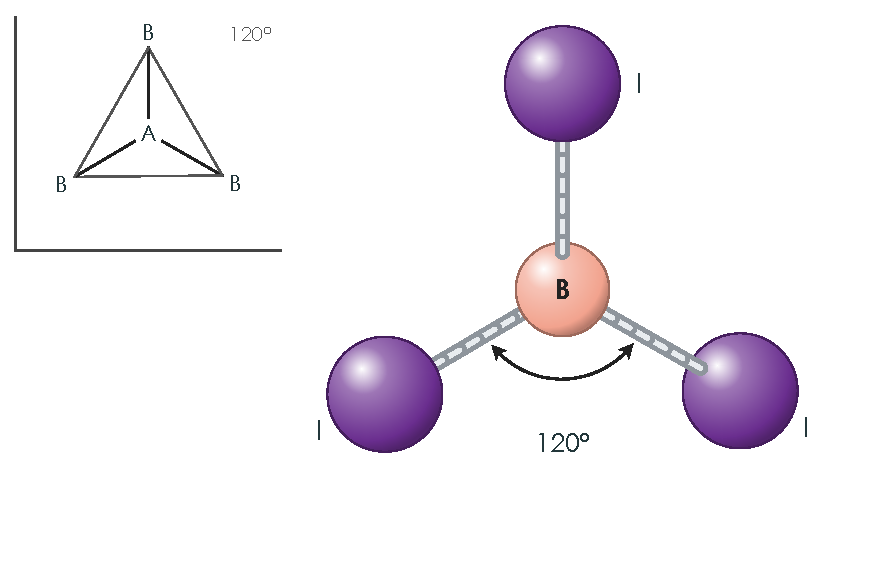
\includegraphics[width=0.6\linewidth]{FigurasSVG/UD3_Enlace_Quimico/pdf/UD3_19_geometria_trigonal_BI3.pdf}
            \caption{Geometría de la molécula \ch{BI3}}
            \label{fig:trigonalBI3}
        \end{figure}
        \item \negrita{Molécula del tipo \ch{AB4}}: son moléculas con geometría \azuln{tetraédrica} con ángulos de enlace de \rojo{\ang{109.5}}.
        Ejemplos: \ch{CH4}, \ch{NH4^+}, \ch{Cl4}, \ch{SO4^{2-}}.
        \begin{figure}[H]
            \centering
            % [FIGURA ORIGINAL] \includegraphics[scale=0.5]{images/imagesUD3EnlaceQuimico/UD3_Teoria/tetraedrica_CCl4}
            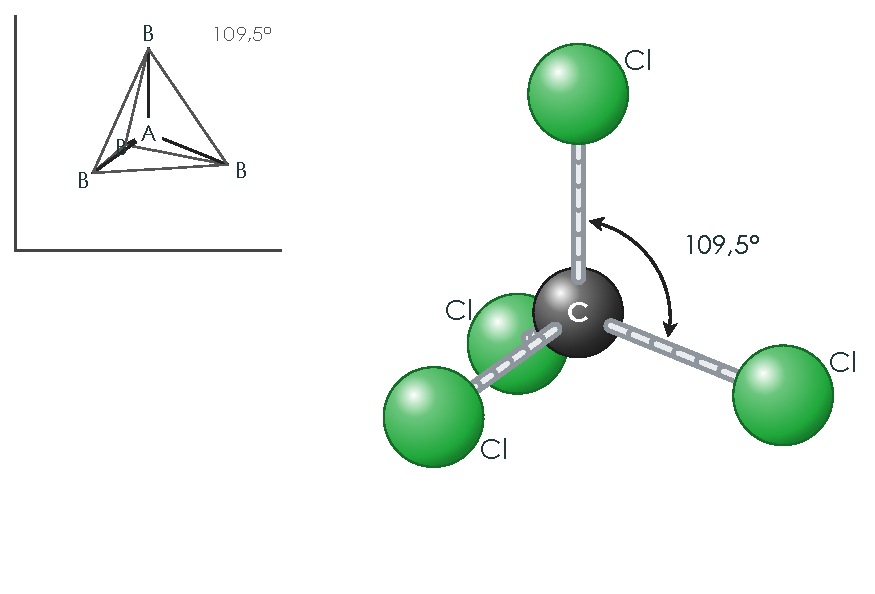
\includegraphics[width=0.6\linewidth]{FigurasSVG/UD3_Enlace_Quimico/pdf/UD3_20_geometria_tetraedrica_CCl4.pdf}
            \caption{Geometría de la molécula \ch{CCl4}}
            \label{fig:geometriaccl4}
        \end{figure}
        \item \negrita{Molécula del tipo \ch{AB5}}: tienen geometría \azuln{bipirámide trigonal}.
        Coexisten dos ángulos tipos de ángulos, unos de \rojo{\ang{120}} y otros de \rojo{\ang{90}}.
        Ejemplos: Ejemplo: \ch{PCl5}
        \begin{figure}[H]
            \centering
            % [FIGURA ORIGINAL] \includegraphics[scale=0.5]{images/imagesUD3EnlaceQuimico/UD3_Teoria/bipiramidetrigonal_PCl5}
            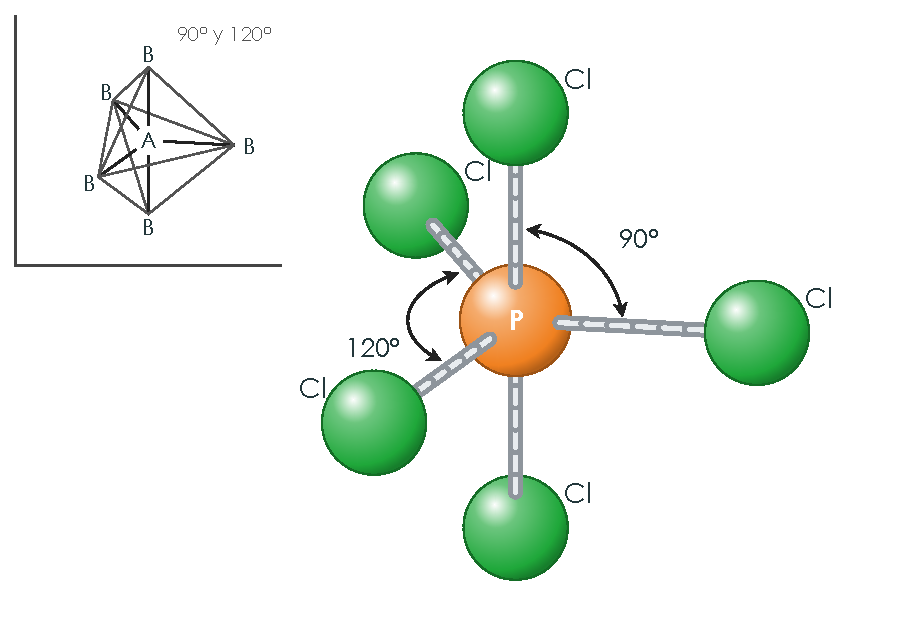
\includegraphics[width=0.6\linewidth]{FigurasSVG/UD3_Enlace_Quimico/pdf/UD3_21_geometria_bipiramide_PCl5.pdf}
            \caption{Geometría de la molécula \ch{PCl5}}
            \label{fig:GeometriadelPCl5}
        \end{figure}
        \item \negrita{Molécula del tipo \ch{AB6}}: son moléculas con geometría \azuln{octaédrica} con ángulos de enlace de \rojo{\ang{90}}.
        Ejemplos: \ch{SF6}
        \begin{figure}[H]
            \centering
            % [FIGURA ORIGINAL] \includegraphics[scale=0.5]{images/imagesUD3EnlaceQuimico/UD3_Teoria/octaedrica_SF6}
            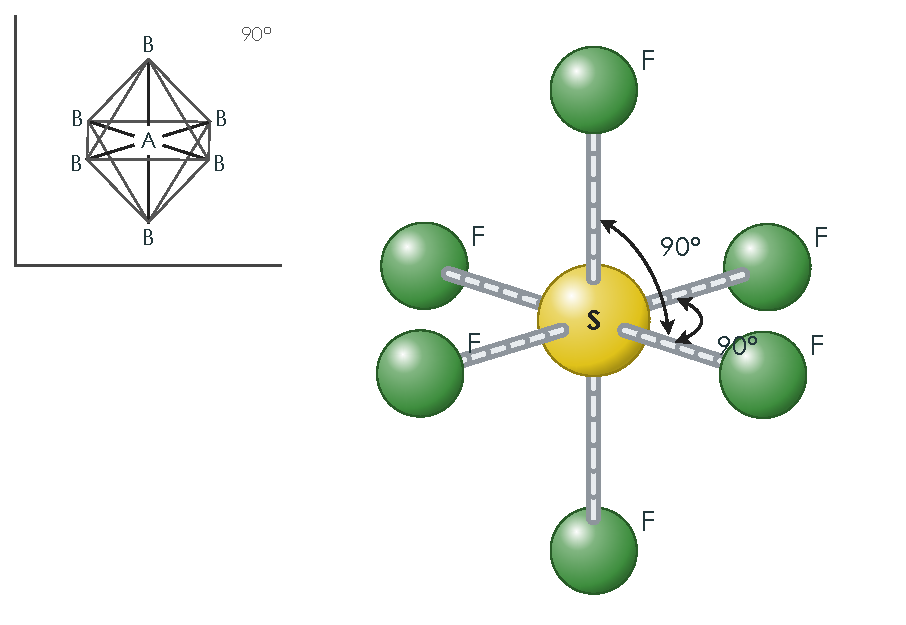
\includegraphics[width=0.6\linewidth]{FigurasSVG/UD3_Enlace_Quimico/pdf/UD3_22_geometria_octaedrica_SF6.pdf}
            \caption{Geometría de la molécula \ch{SF6}}
            \label{fig:GeometriadelamoleculaSF6}
        \end{figure}
\end{enumerate}

\subsubsection[Geometría con pares de electrones no enlazantes]{Geometría de moléculas cuyo átomo central tiene pares de electrones no compartidos o solitarios}
La presencia de pares no enlazantes en una molécula varía el ángulo de enlace por efecto de la repulsión electrónica y por lo tanto modifica su geometría molecular.
Los ángulos disminuyen a medida de que aumenta el número de pares de electrones no enlazantes o no compartidos.

Si usamos el símbolo X para describir los pares de electrones no enlazantes del átomo central, la fórmula general de estas moléculas será: \ch{AB_nX_m}.

\begin{enumerate}[label=\numberballmDarkTeal]
        \item \negrita{Molécula del tipo \ch{AB2X}}: son moléculas con geometría \azuln{angular} y tienen un ángulo de enlace \verden{menor} de \rojon{\ang{120}}.
        Ejemplos: \ch{SO2}, \ch{O3}, \ch{NO2-}, \ch{SnCl2}, \ch{IBr2-}, \ch{ClO2-}.
        \begin{figure}[H]
            \centering
            % [FIGURA ORIGINAL] \includegraphics[scale=0.5]{images/imagesUD3EnlaceQuimico/UD3_Teoria/angular_O3}
            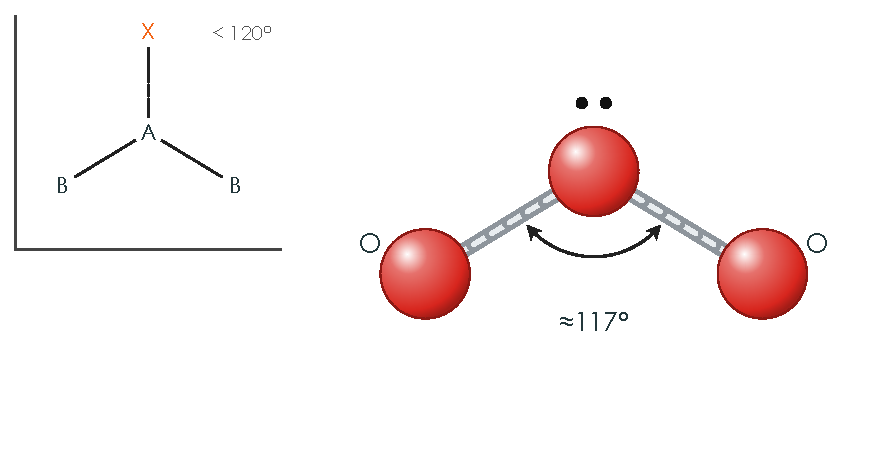
\includegraphics[width=0.6\linewidth]{FigurasSVG/UD3_Enlace_Quimico/pdf/UD3_23_geometria_angular_O3.pdf}
            \caption{Geometría de la molécula \ch{O3}}
            \label{fig:GeometriadelamoleculaO3}
        \end{figure}
        \item \negrita{Molécula del tipo \ch{AB3X}}: son moléculas con una geometría de \azuln{pirámide trigonal}, con ángulos de enlace \verden{menores} de  \rojon{\ang{109.5}}.
        Ejemplos: \ch{NH3}, \ch{H3O+}, \ch{AsH3}, \ch{PH3}, \ch{NF2}, \ch{PBr3}, \ch{PF3}, \ch{ClO3-}.
        \begin{figure}[H]
            \centering
            % [FIGURA ORIGINAL] \includegraphics[scale=0.5]{images/imagesUD3EnlaceQuimico/UD3_Teoria/priamidetrigonal_NH3}
            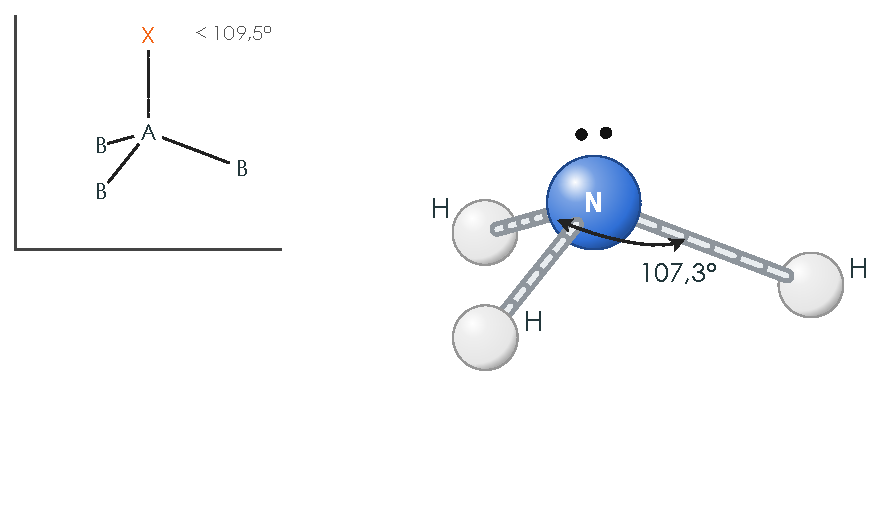
\includegraphics[width=0.6\linewidth]{FigurasSVG/UD3_Enlace_Quimico/pdf/UD3_24_geometria_piramide_NH3.pdf}
            \caption{Geometría de la molécula \ch{NH3}}
            \label{fig:geometriaNH3}
        \end{figure}
        \item \negrita{Molécula del tipo \ch{AB2X2}}: son moléculas con geometría \azuln{angular} con ángulos de enlace \verden{menor} de \rojo{\ang{120}}.
        Ejemplos: \ch{H2O}, \ch{H2S}, \ch{SF2}.
        \begin{figure}[H]
            \centering
            % [FIGURA ORIGINAL] \includegraphics[scale=0.5]{images/imagesUD3EnlaceQuimico/UD3_Teoria/angular_H2S}
            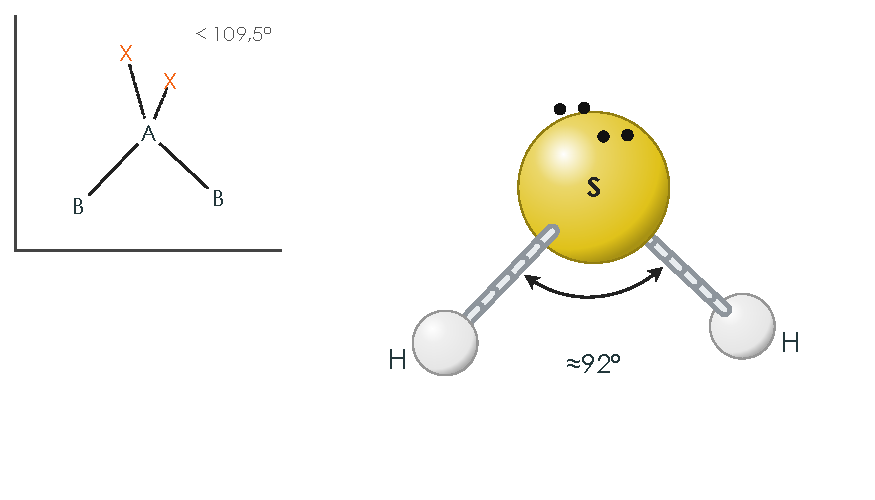
\includegraphics[width=0.6\linewidth]{FigurasSVG/UD3_Enlace_Quimico/pdf/UD3_25_geometria_angular_H2S.pdf}
            \caption{Geometría de la molécula \ch{H2S}}
            \label{fig:geometriaH2S}
        \end{figure}
\end{enumerate}


A modo de resumen en la siguiente tabla se incluyen todos los casos.

%    \begin{longtblr}[
%        caption = {Tabla resumen de la geometría según la TRPECV},
%    ]
%    {
%        colspec = {|Q[c,m]|Q[c,m]|Q[c,m]|Q[c,m]|Q[c,m]|},
%        rowhead = 1,
%        row{1} = {bg=mybluecolour, fg = white, font=\sffamily},
%        vlines = {1}{white},
%    }
%        \hline
%        {\textbf{nº total de} \\ \textbf{pares de \el}}                  & {\textbf{nº total de pares} \\ \textbf{de \el enlazantes}} & {\textbf{nº total de pares} \\ \textbf{de \el no enlazantes}}                   & \textbf{Geometría} & \textbf{Ejemplo} \\
%        \hline
%        2 & 2 & 0 & {\includegraphics[scale=.5]{images/imagesUD3EnlaceQuimico/UD3_Teoria/lineal.png}                                                      Lineal}                       & \ch{BeF2}  \\
%        \hline
%        \SetCell[r=2]{m} 3                   & 3 & 0 & {\includegraphics[scale=.5]{images/imagesUD3EnlaceQuimico/UD3_Teoria/trigonal.png}                                                     Trigonal plana (triangular)} & \ch{BF3}  \\
%        \hline
%        & 2 & 1 & {\includegraphics[scale=.5]{images/imagesUD3EnlaceQuimico/UD3_Teoria/angular.png} Angular   }                                  & \ch{SnCl2}   \\
%        \hline
%        \SetCell[r=3]{m} 4 & 4 & 0 & {\includegraphics[scale=.5]{images/imagesUD3EnlaceQuimico/UD3_Teoria/tetraedrica.png} Tetraédrica }                                                                 & \ch{CH4}   \\
%        \hline
%        & 3 & 1 & {\includegraphics[scale=.5]{images/imagesUD3EnlaceQuimico/UD3_Teoria/piramidetrigonal.png} Pirámide trigonal }                                                      & \ch{NH3}   \\
%        \hline
%        & 2 & 2 & {\includegraphics[scale=.5]{images/imagesUD3EnlaceQuimico/UD3_Teoria/angularb.png} Angular }                           & \ch{H2O}  \\
%        \hline
%        \SetCell[r=4]{m} 5                   & 5 & 0 & {\includegraphics[scale=.5]{images/imagesUD3EnlaceQuimico/UD3_Teoria/bipiramidetrigonal.png} Bipirámide triangular}                                     & \ch{PCl5}  \\
%        \hline
%        & 4 & 1 & {\includegraphics[scale=.5]{images/imagesUD3EnlaceQuimico/UD3_Teoria/tetraedricadistorsionada.png} Tetraédrica distorsionada}                                       & \ch{SF4}   \\
%        \hline
%        & 3 & 2 & {\includegraphics[scale=.5]{images/imagesUD3EnlaceQuimico/UD3_Teoria/enformadeT.png} En forma de T  }                                                               & \ch{ClF3}  \\
%        \hline
%        & 2 & 3 & {\includegraphics[scale=.5]{images/imagesUD3EnlaceQuimico/UD3_Teoria/linealb.png} Lineal  }                       & \ch{XeF2}  \\
%        \hline
%        \SetCell[r=3]{m}6                   & 6 & 0 & {\includegraphics[scale=.5]{images/imagesUD3EnlaceQuimico/UD3_Teoria/octaedrica.png} Octaédrica}                       & \ch{SF6}  \\
%        \hline
%        & 5 & 1 & {\includegraphics[scale=.5]{images/imagesUD3EnlaceQuimico/UD3_Teoria/piramidalcuadrada.png} Pirámide cuadrada}                       & \ch{ICl5}  \\
%        \hline
%        & 4 & 2 & {\includegraphics[scale=.5]{images/imagesUD3EnlaceQuimico/UD3_Teoria/planacuadrada.png} Plano cuadrada}                       & \ch{XeF4}  \\
%        \hline
%    \end{longtblr}

\begin{longtblr}[
    caption = {Tabla resumen de la geometría según la TRPECV},
]
{
    colspec = {|Q[c,m]|Q[c,m]|Q[c,m]|Q[c,m]|Q[c,m]|},
    rowhead = 1,
    row{1} = {bg=mybluecolour, fg = white, font=\sffamily},
    vlines = {1}{white},
}
    \hline
    {\textbf{nº total de} \\ \textbf{pares de \el}}                  & {\textbf{nº total de pares} \\ \textbf{de \el enlazantes}} & {\textbf{nº total de pares} \\ \textbf{de \el no enlazantes}}                   & \textbf{Geometría} & \textbf{Ejemplo} \\
    \hline
    2 & 2 & 0 & Lineal                 & \ch{BeF2}   \\
    \hline
    \SetCell[r=2]{m} 3                   & 3 & 0 & Trigonal plana (triangular)           & \ch{BF3}   \\
    \hline
    & 2 & 1 & Angular                     & \ch{SnCl2}   \\
    \hline
    \SetCell[r=3]{m} 4 & 4 & 0 & Tetraédrica       & \ch{CH4}  \\
    \hline
    & 3 & 1 & Pirámide trigonal   & \ch{NH3}   \\
    \hline
    & 2 & 2 & Angular               & \ch{H2O}  \\
    \hline
    \SetCell[r=4]{m} 5                   & 5 & 0 & Bipirámide triangular                      & \ch{PCl5}  \\
    \hline
    & 4 & 1 & Tetraédrica distorsionada                  & \ch{SF4}   \\
    \hline
    & 3 & 2 & En forma de T           & \ch{ClF3}  \\
    \hline
    & 2 & 3 & Lineal              & \ch{XeF2}  \\
    \hline
    \SetCell[r=3]{m}6                   & 6 & 0 & Octaédrica              & \ch{SF6}  \\
    \hline
    & 5 & 1 & Pirámide cuadrada              & \ch{ICl5}  \\
    \hline
    & 4 & 2 & Plano cuadrada              & \ch{XeF4}  \\
    \hline
\end{longtblr}


\begin{ejemplo}
    \textbf{Indica la geometría molecular de los compuestos \ch{SF2}, \ch{SF4}, \ch{SF6} según la TRPECV.}
    \vspace*{6pt}

    En general para resolver este tipo de ejercicios, deberemos seguir los siguientes pasos:

    \begin{enumerate}
        \item Realizar la estructura de lewis de la molécula.
        \item Contabilizar el número de pares de electrones enlazantes, no enlazantes y pares de electrones totales alrededor del átomo central.
        \item Asignar la geometría según la taba dada anteriormente.
    \end{enumerate}

    \begin{itemize}
        \item \ch{SF2}.
        \begin{itemize}
            \item Estructura de Lewis:

            % [FIGURA ORIGINAL] \includegraphics[scale=1]{images/imagesUD3EnlaceQuimico/UD3_Teoria/ejemplo3_1}
            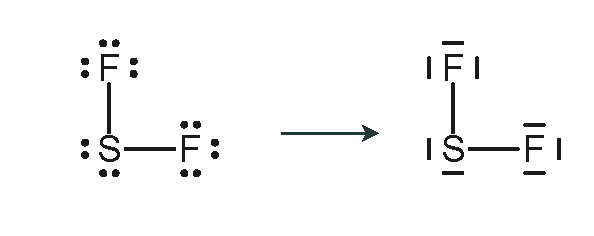
\includegraphics[width=0.4\linewidth]{FigurasSVG/UD3_Enlace_Quimico/pdf/UD3_26_ejemplo_SF2.pdf}

            \item Contabilización del número de pares de electrones.
            \begin{itemize}
                \item Pares de electrones totales = 4
                \item Pares de electrones no enlazantes = 2
                \item Pares de electrones enlazantes = 2
            \end{itemize}
            \item La geometría será en este caso \textbf{angular}.
        \end{itemize}

        \item \ch{SF4}

        \begin{itemize}
            \item Estructura de Lewis:

            % [FIGURA ORIGINAL] \includegraphics[scale=1]{images/imagesUD3EnlaceQuimico/UD3_Teoria/ejemplo3_1_b}
            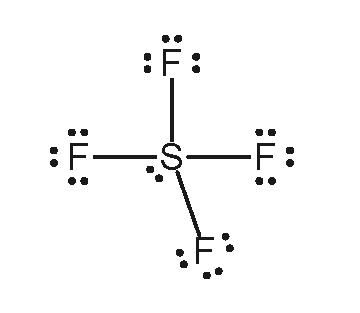
\includegraphics[width=0.25\linewidth]{FigurasSVG/UD3_Enlace_Quimico/pdf/UD3_27_ejemplo_SF4.pdf}

            \item Contabilización del número de pares de electrones.
            \begin{itemize}
                \item Pares de electrones totales = 5
                \item Pares de electrones no enlazantes = 1
                \item Pares de electrones enlazantes = 4
            \end{itemize}
            \item La geometría será en este caso \textbf{tetraédrica distorsionada}.
        \end{itemize}

        \item \ch{SF6}

        \begin{itemize}
            \item Estructura de Lewis:

            % [FIGURA ORIGINAL] \includegraphics[scale=1]{images/imagesUD3EnlaceQuimico/UD3_Teoria/ejemplo3_1_c}
            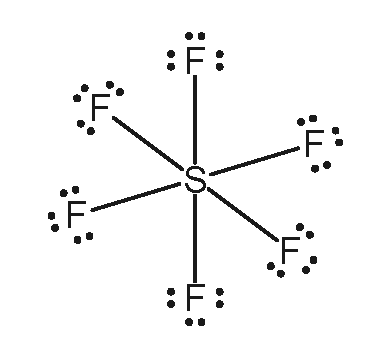
\includegraphics[width=0.27\linewidth]{FigurasSVG/UD3_Enlace_Quimico/pdf/UD3_28_ejemplo_SF6.pdf}

            \item Contabilización del número de pares de electrones.
            \begin{itemize}
                \item Pares de electrones totales = 6
                \item Pares de electrones no enlazantes = 0
                \item Pares de electrones enlazantes = 6
            \end{itemize}
            \item La geometría será en este caso \textbf{octaédrica}.
        \end{itemize}

    \end{itemize}

\end{ejemplo}

\subsection{Teoría del enlace de valencia (TEV)}\label{subsec:teoria-del-enlace-de-valencia-(tev)}

En la sección anterior, hemos visto como la TRPECV nos permitía explicar la geometría de la molécula analizando la disposición de los pares de electrones del átomo central, pero ¿en qué orbitales se sitúan esos electrones?

Para resolver este y otros problemas \textbf{Linus Pauling} propuso la teoría del enlace de valencia.

\begin{center}
    \begin{definicion}[width=0.9\textwidth]{Enlace covalente}
        Un enlace covalente es el solapamiento de un orbital de un átomo con otro orbital de otro átomo, de modo que en los dos orbitales solapados existan dos electrones con sus momentos de \textit{spin} apareados
    \end{definicion}
\end{center}


\begin{figure}[H]
    \centering
    % [FIGURA ORIGINAL] \includegraphics[scale=1]{images/imagesUD3EnlaceQuimico/UD3_Teoria/F2TEV}
    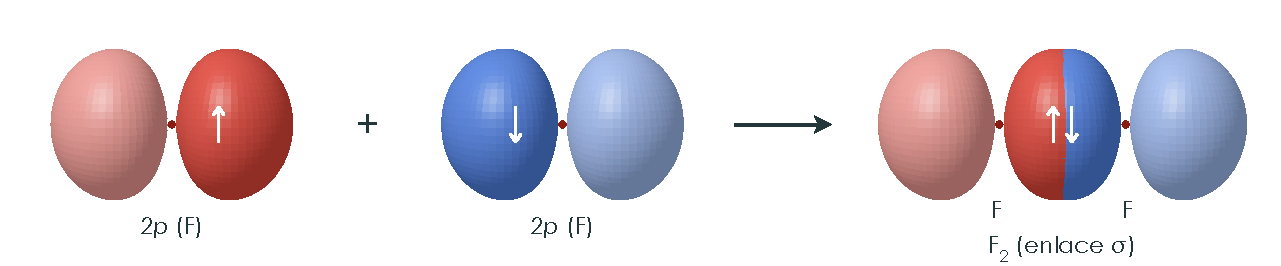
\includegraphics[width=0.8\linewidth]{FigurasSVG/UD3_Enlace_Quimico/pdf/UD3_29_F2_TEV_orbitales.pdf}
    \caption{Los orbitales se aproximan en la orientación adecuada. Se forma un enlace entre los dos átomos de flúor.}\label{fig:f2tev}
\end{figure}

Según el tipo de solapamiento, podemos encontrar dos tipos de enlace:
\begin{enumerate}
    \item \negsubro{Enlace tipo sigma ($\sigma$)}.
    Si ambos orbitales se solapan frontalmente, es decir, en el eje internuclear.
    Ejemplos: orbital $s$ con orbital $s$ (\chemfig{H-H}), orbital $s$ con orbital $p$ (\chemfig{H-Cl}) o orbital $p$ con orbital $p$ (\chemfig{Cl-Cl}).
    \begin{figure}[H]
        \centering
        % [FIGURA ORIGINAL] \includegraphics[scale=0.5]{images/imagesUD3EnlaceQuimico/UD3_Teoria/enlacesigma}
        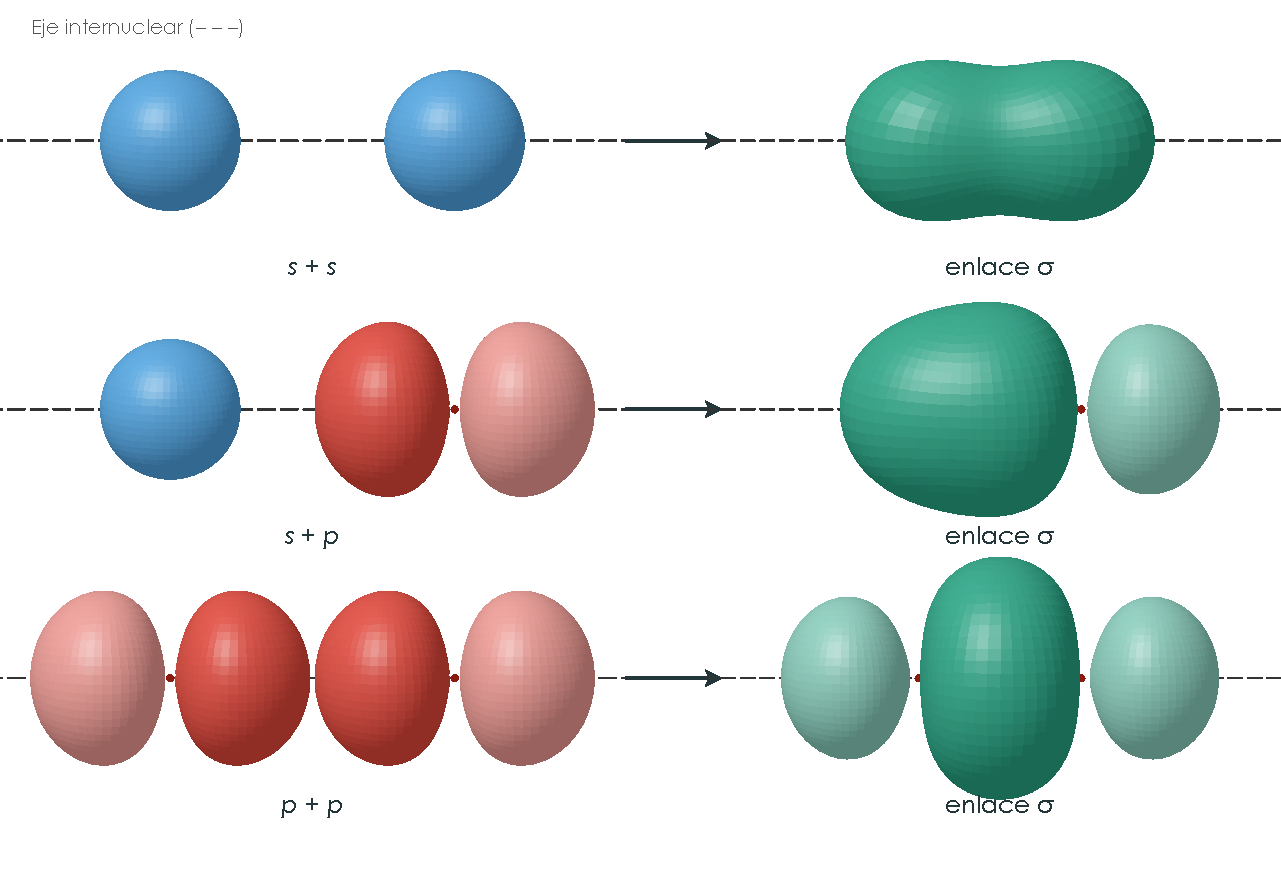
\includegraphics[width=0.8\linewidth]{FigurasSVG/UD3_Enlace_Quimico/pdf/UD3_30_enlace_sigma.pdf}
        \caption{Enlace sigma}
        \label{fig:enlacesigma}
    \end{figure}
    \item \negsubro{Enlace tipo pi ($\pi$)}.
    Se produce cuando el solapamiento es lateral, es decir, a cada lado de la línea internuclear es decir $p_y$ con $p_y$, $p_z$ con $p_z$, $p_y$ con $d$.
    \begin{figure}[H]
        \centering
        % [FIGURA ORIGINAL] \includegraphics[scale=0.5]{images/imagesUD3EnlaceQuimico/UD3_Teoria/enlacepi}
        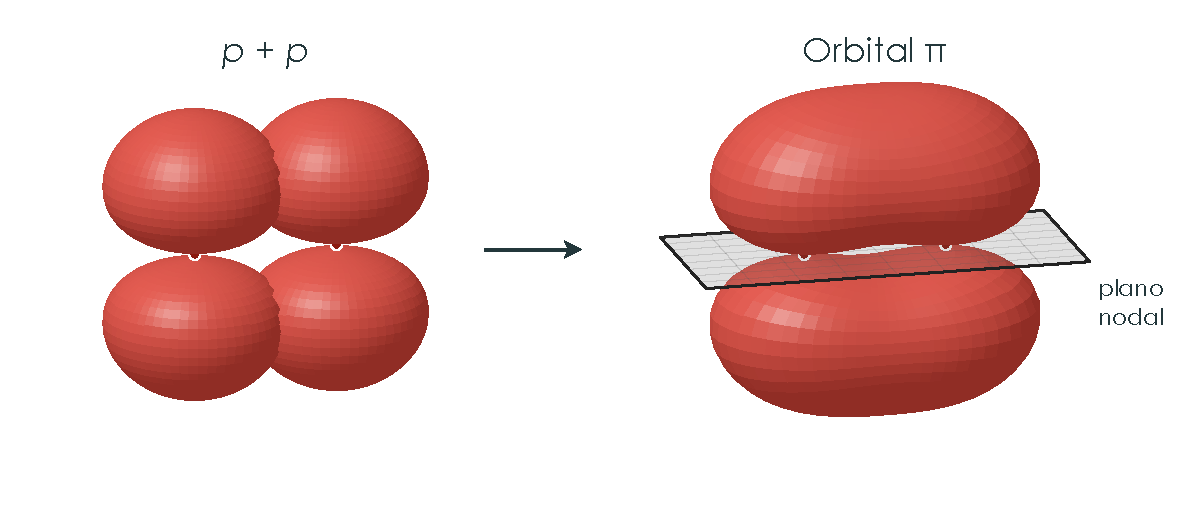
\includegraphics[width=0.75\linewidth]{FigurasSVG/UD3_Enlace_Quimico/pdf/UD3_31_enlace_pi.pdf}
        \caption{Enlace pi}
        \label{fig:enlacepi}
    \end{figure}
\end{enumerate}

Como ejemplos más representativos podemos mencionar:

\begin{enumerate}[label=\numberballmDarkTeal]

        \item \negrita{\ch{H2}}: en este caso, tenemos un solo enlace \(\sigma\) entre los orbitales \(s\) del hidrógeno.

        \begin{figure}[H]
            \centering
            % [FIGURA ORIGINAL] \includegraphics[scale=0.5]{images/imagesUD3EnlaceQuimico/UD3_Teoria/h2tev}
            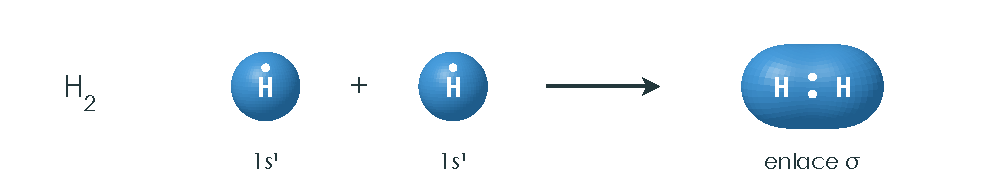
\includegraphics[width=0.7\linewidth]{FigurasSVG/UD3_Enlace_Quimico/pdf/UD3_32_H2_TEV_orbitales.pdf}
            % [FIGURA ORIGINAL] \includegraphics[scale=0.5]{images/imagesUD3EnlaceQuimico/UD3_Teoria/H2tev2}
            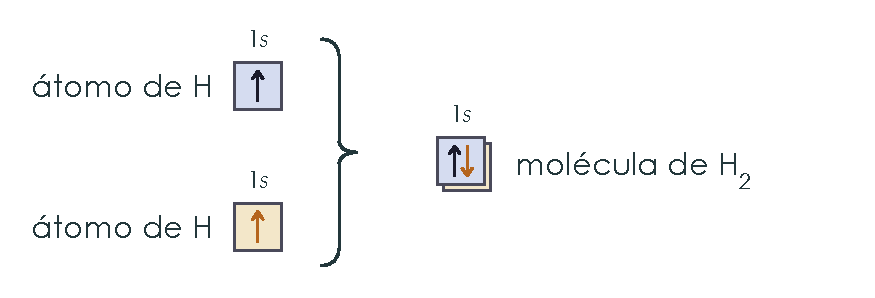
\includegraphics[width=0.55\linewidth]{FigurasSVG/UD3_Enlace_Quimico/pdf/UD3_33_H2_TEV_cajas.pdf}
            \caption{Enlace de \ch{H2} según TEV}
            \label{fig:h2tev}
        \end{figure}

        \item \negrita{\ch{HF}}: en este caso tenemos un enlace \(\sigma\) entre un orbital \(s\) del hidrógeno y un orbital \(p\) del flúor.

        \begin{figure}[H]
            \centering
            % [FIGURA ORIGINAL] \includegraphics[scale=0.5]{images/imagesUD3EnlaceQuimico/UD3_Teoria/HFtev}
            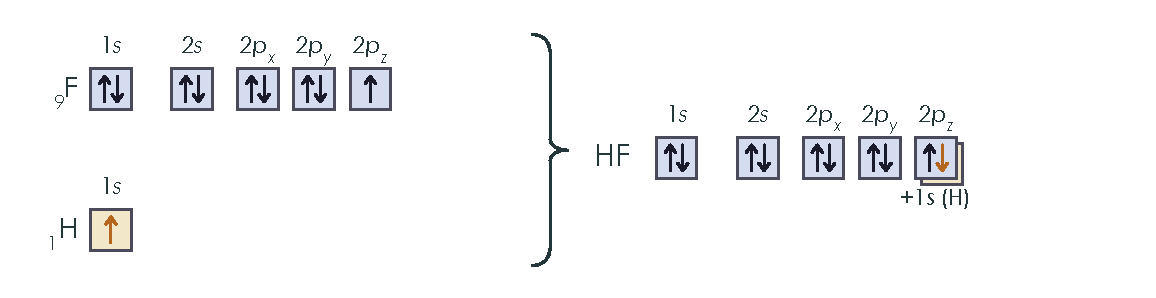
\includegraphics[width=0.75\linewidth]{FigurasSVG/UD3_Enlace_Quimico/pdf/UD3_34_HF_TEV_cajas.pdf}
            \caption{Enlace de \ch{HF} según TEV}
            \label{fig:hftev}
        \end{figure}
        \item \negrita{\ch{H2O}}:en este caso tenemos dos enlaces \(\sigma\) entre un orbital \(p\) del oxígeno y el orbital \(s\)
        \begin{figure}[H]
            \centering
            % [FIGURA ORIGINAL] \includegraphics[scale=0.5]{images/imagesUD3EnlaceQuimico/UD3_Teoria/H2Otev}
            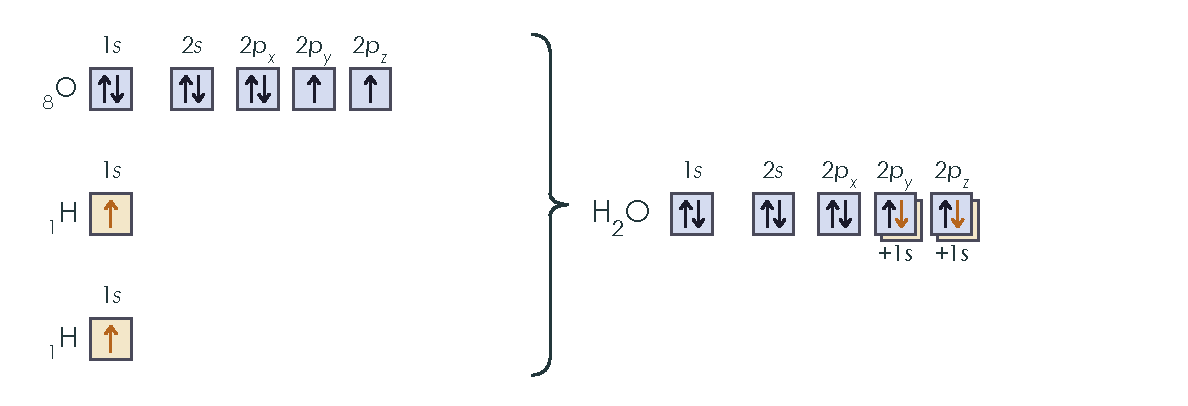
\includegraphics[width=0.75\linewidth]{FigurasSVG/UD3_Enlace_Quimico/pdf/UD3_35_H2O_TEV_cajas.pdf}
            \caption{Enlace de \ch{H2O} según TEV}
            \label{fig:h2otev}
        \end{figure}
        \item \negrita{\ch{O2}}: este es un caso más complejo, en el que tenemos un enlace \(\sigma\) entre los dos orbitales \(p\) de cada átomo de oxígeno y dos enlaces \(\pi\) entre dos orbitales \(p\) de cada átomo de oxígeno.
        \begin{figure}[H]
            \centering
            % [FIGURA ORIGINAL] \includegraphics[scale=0.5]{images/imagesUD3EnlaceQuimico/UD3_Teoria/o2tev}
            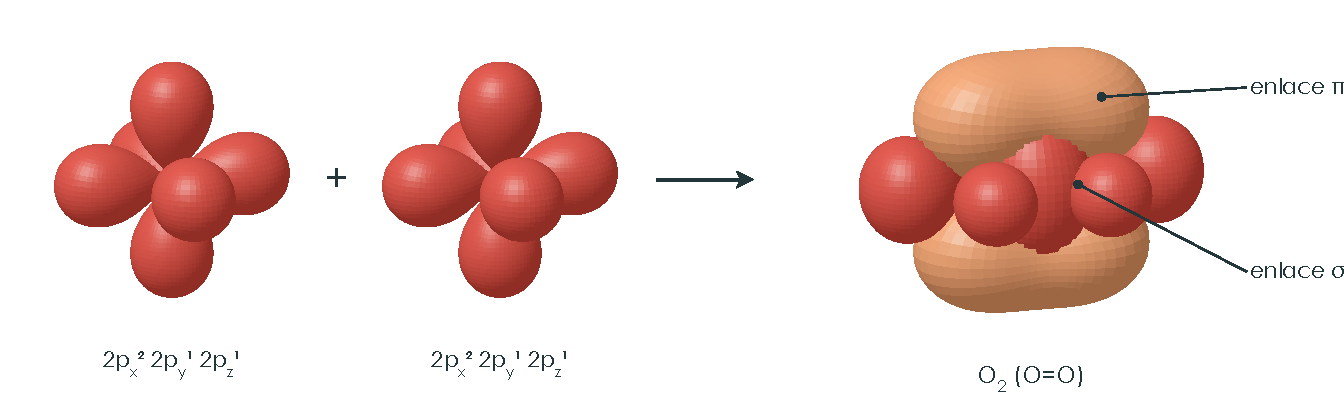
\includegraphics[width=0.85\linewidth]{FigurasSVG/UD3_Enlace_Quimico/pdf/UD3_36_O2_TEV_orbitales.pdf}
            \caption{Enlace de \ch{O2} según TEV}
            \label{fig:o2tev}
        \end{figure}

        Sabemos también que existen moléculas que puede formar cuatro en incluso 6 enlaces covalentes (\ch{SO2}, \ch{SO3}, \ch{H2SO4}, \ch{SF6}). Estos enlaces los explicaba la teoría de Lewis con las excepciones del octeto expandido.
        Para explicarlo según la teoría del enlace de valencia, tenemos que tener en cuenta que a partir del tercer periodo existen orbitales $d$ que pueden estar vacíos y por tanto se puede producir una expansión de unos de los electrones a estos orbitales, tal y como se muestra en la siguiente figura.
        \begin{figure}[H]
            \centering
            % [FIGURA ORIGINAL] \includegraphics[scale=0.5]{images/imagesUD3EnlaceQuimico/UD3_Teoria/soctetotev}
            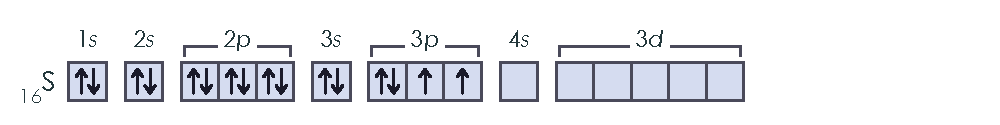
\includegraphics[width=0.75\linewidth]{FigurasSVG/UD3_Enlace_Quimico/pdf/UD3_37_S_covalencia_2.pdf}
            % [FIGURA ORIGINAL] \includegraphics[scale=0.5]{images/imagesUD3EnlaceQuimico/UD3_Teoria/soctetotev2}
            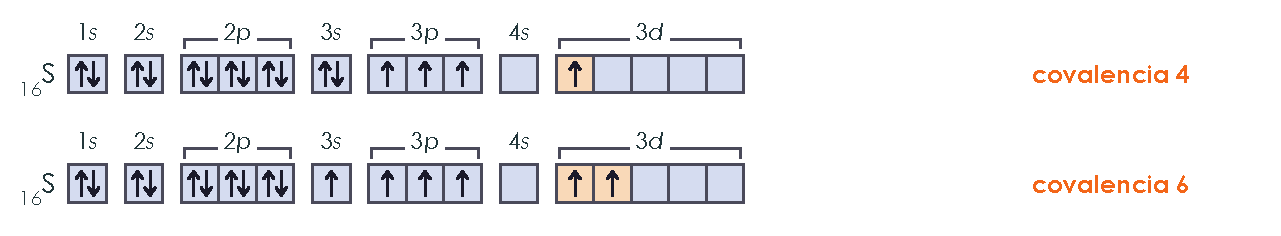
\includegraphics[width=0.85\linewidth]{FigurasSVG/UD3_Enlace_Quimico/pdf/UD3_38_S_covalencias_4_6.pdf}
            \caption{Enlace de \ch{O2} según TEV}
            \label{fig:soctetotev}
        \end{figure}
\end{enumerate}

\subsection{Teoría de los orbitales híbridos atómicos}\label{subsec:teoria-de-los-orbitales-hibridos-atomicos}

La TRPECV no puede explicar la geometría de todas las moléculas así como tampoco podría explicar los ángulos de enlace de algunas moléculas la teoría del enlace de valencia.
La \azuln{teoría de hibridación de orbitales atómicos} resolvía estas cuestiones en la que se propuso que durante la reacción y previa formación del enlace, se produce la hibridación o combinación de los orbitales atómicos puros dando lugar a unos nuevos orbitales híbridos.

\subsubsection{Hibridación: concepto y tipos}

\begin{center}
    \begin{definicion}[width=0.9\textwidth]{Hibridación}
        La \textbf{hibridación} es un proceso mediante el cual orbitales atómicos puros de energía parecida se combinan entre sí, transformándose en otros orbitales denominados \textbf{orbitales atómicos híbridos}.
    \end{definicion}
\end{center}


Los orbitales híbridos se caracterizan por:
\begin{enumerate}[label=\numberballmDarkTeal]
        \item Se forman tantos orbitales híbridos como orbitales atómicos combinados.
        \item Los orbitales híbridos son iguales energéticamente y solo se diferencia en su distribución espacial.
        \item Se disponen en direcciones que facilitan el solapamiento con los orbitales del otro átomo al formar el enlace.
\end{enumerate}

Los tipos de hibridación que nos podemos encontrar son:

\begin{enumerate}[label=\numberballmDarkBrown]
        \item \negsubro{Hibridación $\bm{sp^3}$}.
        Tomaremos como ejemplo el metano \ch{CH4}.
        En este caso los orbitales atómicos que se hibridan son los del carbono.
        El carbono tiene una configuración electrónica: \ch{C}: $\color{blue}{1s^2\;2s^2\;2p_x^1\;2p_y^1\;2p_x^0}$.
        Vemos que uno de los electrones del $2s$ puede promocionar al orbital $2p_z$ vacío quedando una configuración del carbono excitado (se ha producido la promoción de un electrón) \ch{C^*}: $\color{red}{1s^2\;2s^1\;2p_x^1\;2p_y^1\;2p_x^1}$.
        A partir de la combinación de un orbital $s$ (en este caso $2s$) y 3 orbitales $p$ (en este caso $2p$) resultan cuatro orbitales $sp^3$ con una disposición \azuln{tetraédrida} y ángulos de enlace de \rojon{\ang{109.5}}.
        Una vez producida la hibridación del átomo de carbono, se produce el acoplamiento \azuln{frontal} del orbital $s$ del hidrógeno con cada uno de los orbitales $sp^3$ del carbono.
        \begin{figure}[H]
            \centering
            % [FIGURA ORIGINAL] \includegraphics[scale=0.5]{images/imagesUD3EnlaceQuimico/UD3_Teoria/metanosp3}
            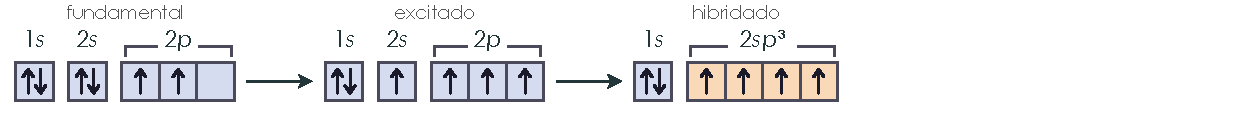
\includegraphics[width=0.85\linewidth]{FigurasSVG/UD3_Enlace_Quimico/pdf/UD3_39_CH4_sp3_cajas.pdf}
            % [FIGURA ORIGINAL] \includegraphics[scale=0.5]{images/imagesUD3EnlaceQuimico/UD3_Teoria/metanosp3_e}
            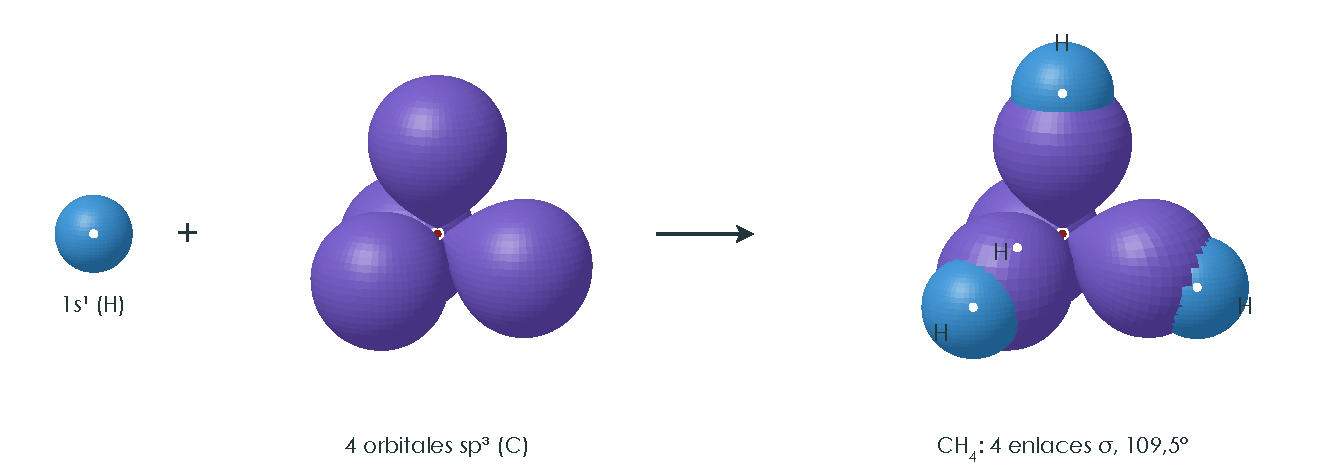
\includegraphics[width=0.85\linewidth]{FigurasSVG/UD3_Enlace_Quimico/pdf/UD3_40_CH4_sp3_orbitales.pdf}
            \caption{Formación del \ch{CH4}}
            \label{fig:formacionmetano}
        \end{figure}

        \caja{Cuando se combinen dos orbitales $sp^3$ o un orbital $s$ con un orbital $sp^3$ se forma un enlace de tipo $\sigma$ debido a que se produce un acoplamiento frontal.}

        \item \negsubro{Hibridación $\bm{sp^2}$}.
        Tomaremos como ejemplo el \ch{BF3}.
        En este caso los orbitales atómicos que se hibridan son los del boro.
        El boro tiene una configuración electrónica: \ch{B}: $\color{blue}{1s^2\;2s^2\;2p_x^1\;2p_y^0\;2p_x^0}$.
        Vemos que \azuln{uno}  de los electrones del $2s$ puede promocionar al orbital $2p_y$ vacío quedando una configuración del boro excitado (se ha producido la promoción de un electrón) \ch{B^*}: $\color{red}{1s^2\;2s^1\;2p_x^1\;2p_y^1\;2p_x^0}$.
        A partir de la combinación de un orbital $s$ (en este caso $2s$) y 2 orbitales $p$ (en este caso $2p_x$ y $2p_y$ ) resultan tres orbitales $sp^2$ con una disposición \azuln{trigonal plana} y ángulos de enlace de \rojon{\ang{120}}.
        Una vez producida la hibridación del átomo de boro, se produce el acoplamiento \azuln{frontal} de los orbitales orbital $p$ del flúor con cada uno de los orbitales $sp^2$ del boro.
        \begin{figure}[H]
            \centering
            % [FIGURA ORIGINAL] \includegraphics[scale=0.75]{images/imagesUD3EnlaceQuimico/UD3_Teoria/BF3sp2}
            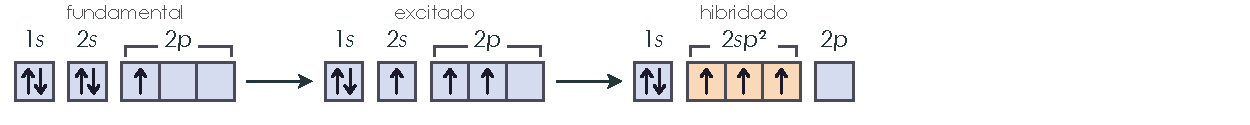
\includegraphics[width=0.85\linewidth]{FigurasSVG/UD3_Enlace_Quimico/pdf/UD3_41_BF3_sp2_cajas.pdf}
            \caption{Formación del \ch{BF3}}
            \label{fig:formacionbf3}
        \end{figure}
        Otro ejemplo sería la formación del \ch{AlCl3}.
        En este caso se hibridaría el átomo de aluminio según:
        \begin{figure}[H]
            \centering
            % [FIGURA ORIGINAL] \includegraphics[scale=0.75]{images/imagesUD3EnlaceQuimico/UD3_Teoria/AlCl3sp2}
            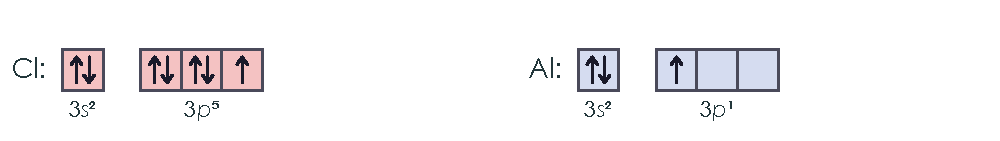
\includegraphics[width=0.7\linewidth]{FigurasSVG/UD3_Enlace_Quimico/pdf/UD3_42_AlCl3_cajas_fundamental.pdf}
            % [FIGURA ORIGINAL] \includegraphics[scale=0.75]{
            % [FIGURA ORIGINAL] images/imagesUD3EnlaceQuimico/UD3_Teoria/AlCl3sp2_b}
            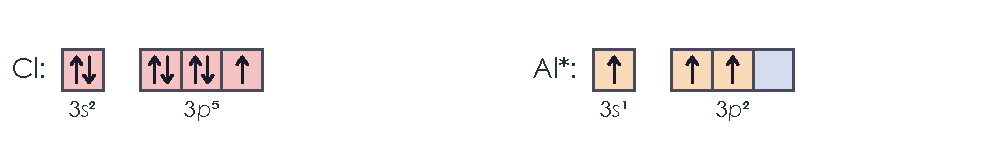
\includegraphics[width=0.7\linewidth]{FigurasSVG/UD3_Enlace_Quimico/pdf/UD3_43_AlCl3_cajas_excitado.pdf}
            \caption{Formación del \ch{AlCl3}}
            \label{fig:formacionalcl3}
        \end{figure}
        En este caso el orbital $3s$ se combina con dos orbitales $2p$ para formar tres orbitales híbridos $sp^2$.
        Estos orbitales híbridos del aluminio se combinarán en este caso con orbitales $p$ del cloro para formar la molécula de \ch{AlCl3}
        \begin{figure}[H]
            \centering
            % [FIGURA ORIGINAL] \includegraphics[scale=0.75]{images/imagesUD3EnlaceQuimico/UD3_Teoria/AlCl3sp2_c}
            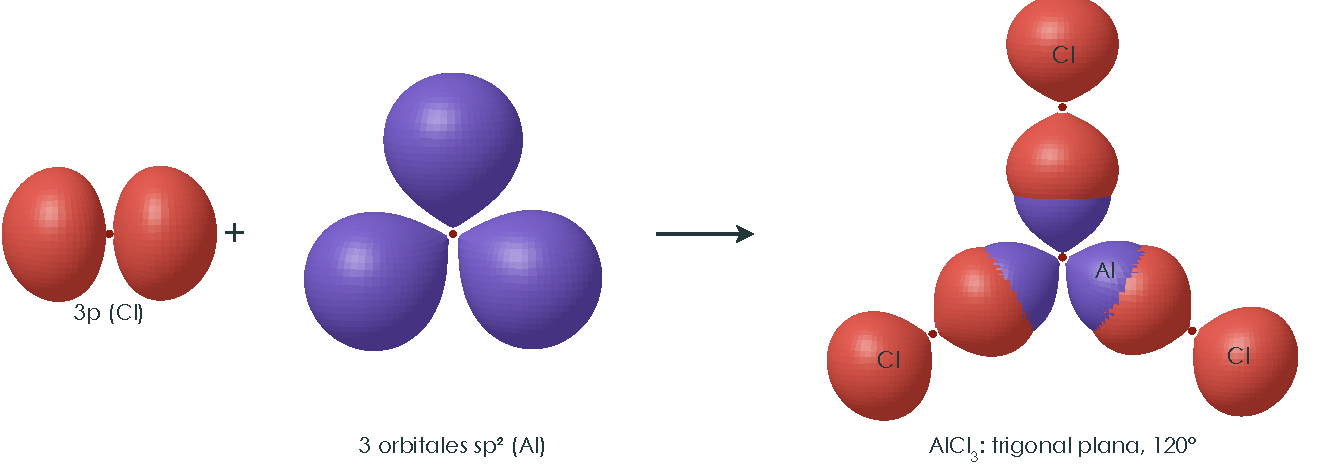
\includegraphics[width=0.85\linewidth]{FigurasSVG/UD3_Enlace_Quimico/pdf/UD3_44_AlCl3_sp2_orbitales.pdf}
            \caption{Formación del \ch{AlCl3}}
            \label{fig:formacionalcl3_b}
        \end{figure}

        \item \negsubro{Hibridación $\bm{sp}$}.
        Tomaremos como ejemplo el \ch{BeF2}.
        En este caso los orbitales atómicos que se hibridan son los del berilio.
        El berilio tiene una configuración electrónica: \ch{B}: $\color{blue}{1s^2\;2s^2\;2p_x^0\;2p_y^0\;2p_x^0}$.
        Vemos que \azuln{uno} de los electrones del $2s$ puede promocionar al orbital $2p_x$ vacío quedando una configuración del berilio excitado (se ha producido la promoción de un electrón) \ch{Be^*}: $\color{red}{1s^2\;2s^1\;2p_x^1\;2p_y^0\;2p_x^0}$.

        \begin{figure}[H]
            \centering
            % [FIGURA ORIGINAL] \includegraphics[scale=0.5]{images/imagesUD3EnlaceQuimico/UD3_Teoria/BeF2sp}
            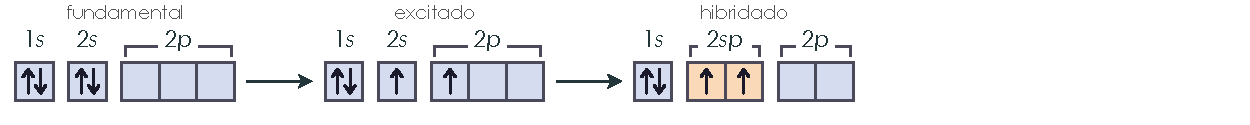
\includegraphics[width=0.85\linewidth]{FigurasSVG/UD3_Enlace_Quimico/pdf/UD3_45_BeF2_sp_cajas.pdf}
            % [FIGURA ORIGINAL] \includegraphics[scale=0.5]{images/imagesUD3EnlaceQuimico/UD3_Teoria/BeF2sp_b}
            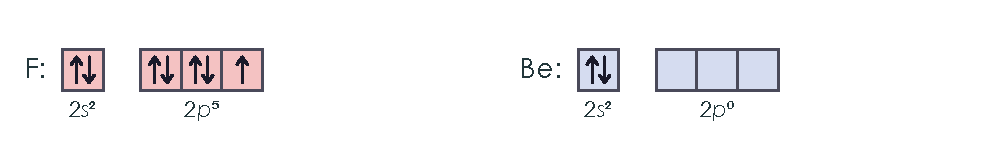
\includegraphics[width=0.7\linewidth]{FigurasSVG/UD3_Enlace_Quimico/pdf/UD3_46_BeF2_cajas_fundamental.pdf}
            % [FIGURA ORIGINAL] \includegraphics[scale=0.5]{images/imagesUD3EnlaceQuimico/UD3_Teoria/BeF2sp_c}
            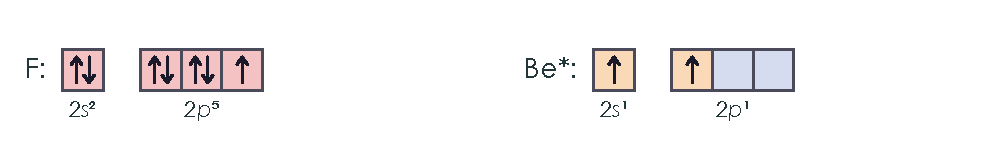
\includegraphics[width=0.7\linewidth]{FigurasSVG/UD3_Enlace_Quimico/pdf/UD3_47_BeF2_cajas_excitado.pdf}
            \caption{Formación del \ch{BeF2}}
            \label{fig:formacionbef2}
        \end{figure}

        A partir de la combinación de un orbital $s$ (en este caso $2s$) y 1 orbital $p$ (en este caso $2p_x$) resultan dos orbitales $sp$ con una disposición \azuln{lineal} y ángulos de enlace de \rojon{\ang{180}}.
        Una vez producida la hibridación del átomo de berilio, se produce el acoplamiento \azuln{frontal} de los orbitales orbital $p$ del flúor con cada uno de los orbitales $sp$ del berilio.

        \begin{figure}[H]
            \centering
            % [FIGURA ORIGINAL] \includegraphics[scale=0.5]{images/imagesUD3EnlaceQuimico/UD3_Teoria/BeF2sp_d}
            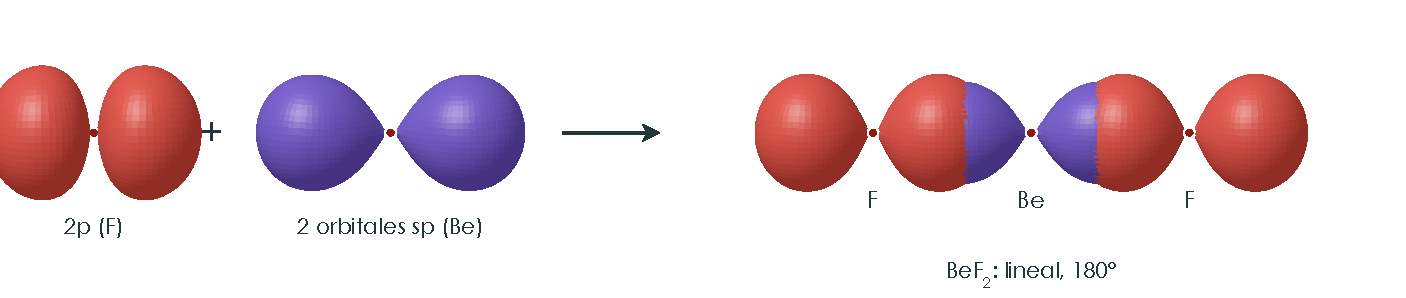
\includegraphics[width=0.85\linewidth]{FigurasSVG/UD3_Enlace_Quimico/pdf/UD3_48_BeF2_sp_orbitales.pdf}
            \caption{Formación del \ch{BeF2}}
            \label{fig:formacionBeF2_b}
        \end{figure}

        \item \negsubro{Hibridación $dsp^2$}.
        A partir de dos orbitales $d$, un orbital $s$ y tres orbitales $p$ resultan cuatro orbitales de un mismo plano formando ángulos \rojon{\ang{90}} entre sí.
        Ejemplos: \ch{Ni(CO)4}

        \item \negsubro{Hibridación $d^2sp^3$}.
        A partir de dos orbitales $d$, un orbital $s$ y tres orbitales $p$ dan lugar a 6 orbitales híbridos $d^2sp^3$.
        Forma una geometría \azuln{octaédrica} con ángulos de enlace \rojon{\ang{90}}.
        Ejemplo: \ch{SF6}.
        \item \negsubro{Hibridación $dsp^3$}.
        A partir de 1 orbital $d$, un orbital $s$ y tres orbitales $p$ dan lugar a 5 orbitales híbridos $dsp^3$.
        Forma una geometría \azuln{bipirámide trigonal} con ángulos de enlace de \rojon{\ang{120}} y \rojon{\ang{90}}.
        Ejemplo: \ch{PCl5}
\end{enumerate}

\subsubsection{Tipos de enlaces entre los orbitales cuando se produce hibridaciones}
Cuando tenemos hibridaciones los enlaces $\sigma$ y enlaces $\pi$ se producen por el acoplamiento de los siguientes tipos de orbitales:
\begin{enumerate}[label=\numberballmDarkTeal]
        \item \negsubro{Enlace $\sigma$}.
        Tendremos un acoplamiento frontal
        \begin{enumerate}
            \item Orbital híbrido -- orbital híbrido siempre y cuando sean del mismo tipo
            \item Cualquier orbital híbrido -- s
            \item Cualquier orbital híbrido -- p
        \end{enumerate}
        \item \negsubro{Enlace $\pi$}.
        Tendremos un acoplamiento lateral.
        Y se produce por acoplamiento de cualquier orbital $p$ siempre y cuando se produzca de manera transversal.
\end{enumerate}

\marcador{Ejercicio}: Explicar los enlaces de las moléculas de \azuln{etano}, \azuln{eteno} y \azuln{etino}

\subsection{Teoría de los orbitales moleculares (OOMM)}\label{subsec:teoria-de-los-orbitales-moleculares-(oomm)}

\caja{Un orbital molecular es una zona en la que es probable que se encuentre un determinado electrón.}

Los orbitales moleculares moleculares se forman por combinaciones lineales de orbitales atómicos.
La combinación de $\bm{n}$ orbitales atómicos producen la formación de $\bm{2n}$ orbitales moleculares teniendo siempre un orbital molecular \azuln{enlazante} (máxima probabilidad de encontrar los electrones) y un orbital molecular \azuln{antienlazante} (mínima probabilidad de encontrar los electrones.).
Los orbitales moleculares se representan mediante su correspondiente función de onda ($\Psi$)
\begin{gather}
    \text{\textbf{Orbital molecular enlazante: }}\quad \Psi_{enlazante} = c_1\Psi_A + c_2\Psi_B\separ
    \text{\textbf{Orbital molecular antienlazante: }}\quad \Psi_{antienlazante} = c_1\Psi_A - c_2\Psi_B
\end{gather}

\subsubsection{Tipos de orbitales moleculares}

Los orbitales moleculares los podemos resumir en dos tipos $\sigma$ y tipo $\pi$
\begin{enumerate}[label=\numberballmDarkTeal]
        \item \negsubro{Orbitales $\sigma$}.
        Se obtienen por interacción frontal de forma similar a lo visto anteriormente y cuando se forman siempre tendremos orbitales $\sigma$ enlazantes representados por $\sigma$ y orbitales $\sigma$ antienlazantes representados por $\sigma^*$.
        \item \negsubro{Orbitales $\pi$}.
        Se obtienen por interacción lateral de forma similar a lo visto anteriormente y cuando se forman siempre tendremos orbitales $\pi$ enlazantes representados por $\pi$ y orbitales $\pi$ antienlazantes representados por $\pi^*$.
\end{enumerate}

\begin{figure}[h]
    \centering
    % [FIGURA ORIGINAL] \includegraphics[scale=0.5]{images/imagesUD3EnlaceQuimico/UD3_Teoria/orbitales_moleculares}
    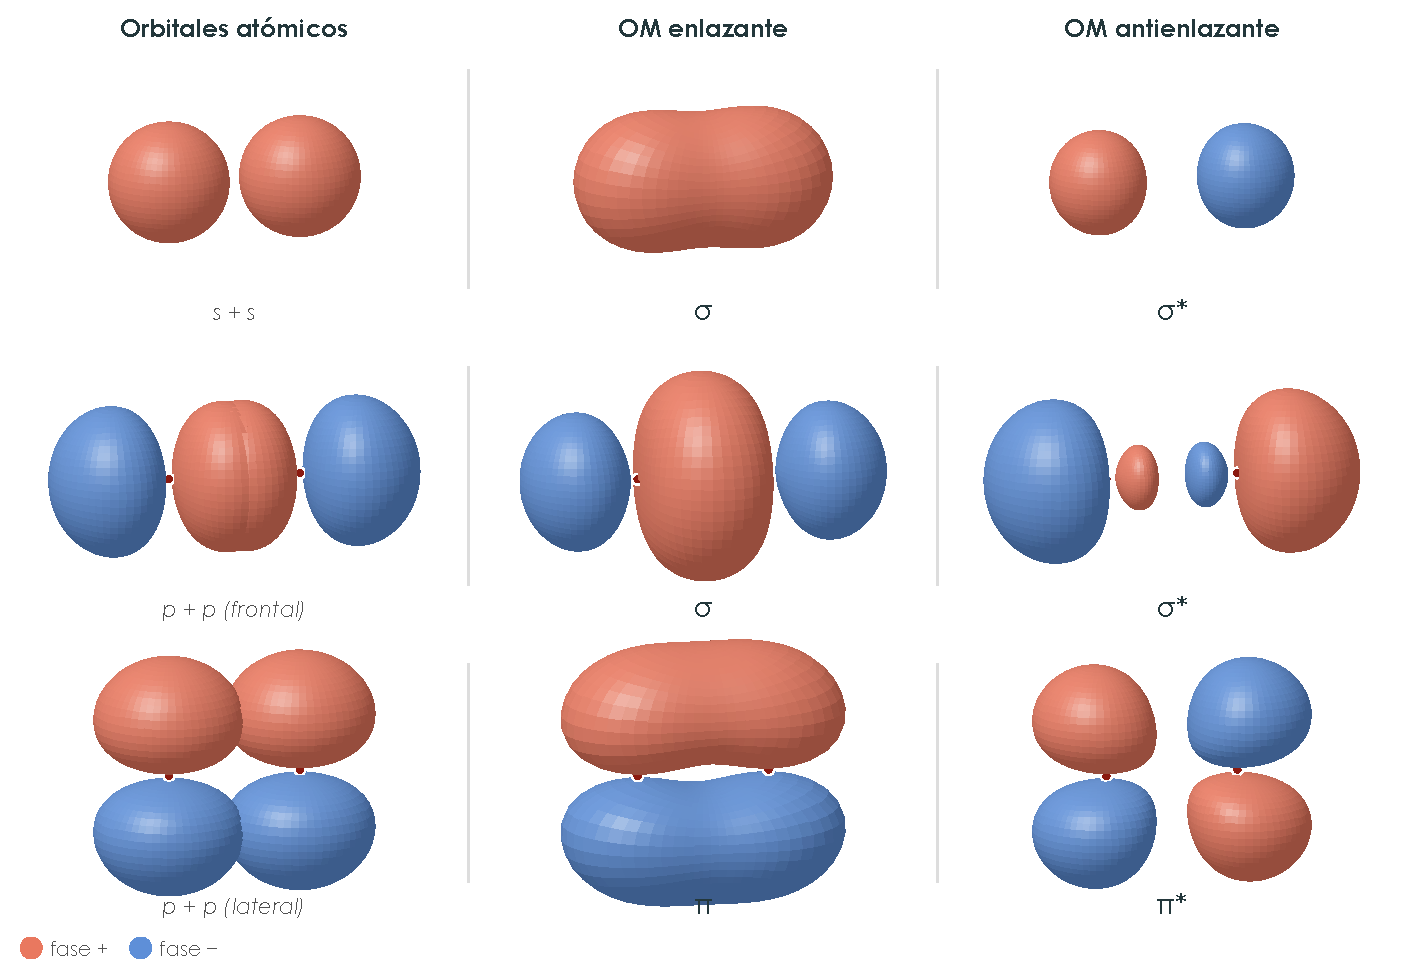
\includegraphics[width=0.85\linewidth]{FigurasSVG/UD3_Enlace_Quimico/pdf/UD3_49_orbitales_moleculares.pdf}
    \caption{(a) Orbitales moleculares $\sigma$ enlazantes y antienlazantes formados a partir de orbitales atómicos $s$ y $p$. (b) orbitales moleculares $\pi$ enlazantes y antienlazantes formados a partir de orbitales atómicos $p$ y $d$}
    \label{fig:Orbitalesatomicos}
\end{figure}

%    \subsection{Diagramas de energía y configuración electrónica}\label{subsec:diagramas-de-energia-y-configuracion-electronica}
%
%    En el caso de moléculas formadas por dos átomos iguales, el orden creciente de energías es, para los dos primeros niveles el siguiente:
%    \begin{figure}[H]
%        \centering
%        \includegraphics[scale=0.5]{images/imagesUD3EnlaceQuimico/UD3_Teoria/diagrama_energia_oomm}
%        \caption{Origen energético moléculas homoatómicas}
%        \label{fig:orgenenergeticooomm}
%    \end{figure}
%
%    A continuación, se muestra el diagrama energético para las moléculas de \ch{H2} y de \ch{O2}.
%
%    \begin{figure}[h]
%        \centering
%        \includegraphics[scale=0.5]{images/imagesUD3EnlaceQuimico/UD3_Teoria/diagrama_oomm_h2}
%        \caption{Diagrama energético OOMM para el \ch{H2}}
%        \includegraphics[scale=0.5]{images/imagesUD3EnlaceQuimico/UD3_Teoria/diagrama_oomm_o2}
%        \caption{Diagrama energético OOMM para el \ch{O2}}
%        \label{fig:Diagramaoommh2yo2}
%    \end{figure}

% \subsection{Propiedades de los compuestos covalentes}

% A diferencia de las sustancias iónicas, las sustancias iónicas tendrán un tipo de propiedades según se enlacen como moléculas discretas o formen redes tridimensionales.

% \begin{enumerate}[label=\numberballmDarkTeal]
%     \item \negsubro{Sustancias moleculares}. Suelen ser moléculas discretas pero que en determinadas ocasiones y en las condiciones ópticas de presión y temperatura pueden formar \azuln{cristales moleculares}
%           \begin{enumerate}
%               \item \negrita{Estado de agregación}. Tienen baja densidad, suelen ser gases o líquidos de bajo punto de ebullición o en algunos casos sólidos blandos de bajo punto de fusión y subliman fácilmente.
%               \item \negrita{Solubilidad}. Dependerá de las fuerzas intermoleculares (se verá más adelante). Las sustancias polares se disolverán en disolventes polares y las sustancias apolares en sustancias apolares (\textit{lo semejante disuelve a lo semejante})
%               \item \negrita{Conductividad eléctrica}. No conducen la electricidad, son buenos \azuln{aislantes}
%           \end{enumerate}
%     \item \negsubro{Sustancias atómicas}. Son sustancias que se agrupan de manera que forman redes moleculares similares a las redes cristalinas de los compuestos iónicos. Ejemplos: grafito, \ch{SiO2}
%           \begin{enumerate}
%               \item \negrita{Estado de agregación}. Suelen ser sólidos de alto punto de fusión y ebullición.
%               \item \negrita{Solubilidad}. Suelen ser insolubles en cualquier disolvente
%               \item \negrita{Conductividad eléctrica}. Son malos conductores de la electricidad con la excepción del grafito.
%           \end{enumerate}
% \end{enumerate}

\subsection{Sólidos covalentes}\label{subsec:solidos-covalentes}

Hay sustancias sólidas formadas por un número indeterminado de átomos unidos mediante un enlace covalente.
Se llaman \textbf{sólidos covalentes}.

Los sólidos covalentes más comunes son el diamante, grafito y la sílice

\begin{enumerate}[label=\numberballmDarkTeal]
        \item El \textbf{diamante} está formado por átomos de carbono con hibridación \(\bm{sp^3}\).
        Cada átomo de carbono está unido a otros cuatro átomos mediante enlaces covalentes.
        Es el material más duro que existe teniendo por tanto también un elevado \textbf{punto de fusión}.
        \begin{figure}[H]
            \centering
            % [FIGURA ORIGINAL] \includegraphics[scale=0.2]{images/imagesUD3EnlaceQuimico/UD3_Teoria/diamante}
            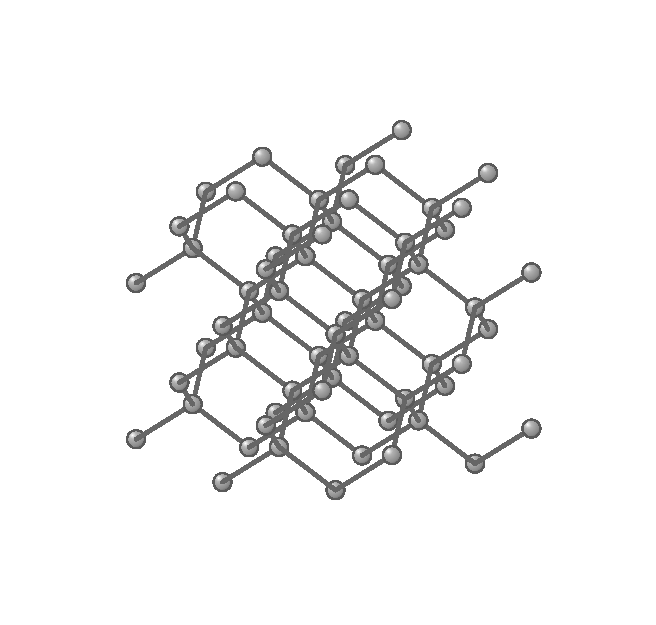
\includegraphics[width=0.45\linewidth]{FigurasSVG/UD3_Enlace_Quimico/pdf/UD3_50_diamante.pdf}
            \caption{Estructura atómica del diamante}\label{fig:diamante}
        \end{figure}
        \item El \textbf{grafito} está formado por carbono con una hibridación \(\bm{sp^2}\).
        Forma anillos planos con una geometría trigonal plana.
        Los electrones que están en los orbitales \(\bm{p}\) perpendiculares al plano forman una nube \(\bm{\pi}\) que permite la conductividad eléctrica.

        \begin{figure}[H]
            \centering
            % [FIGURA ORIGINAL] \includegraphics[scale=1.6]{images/imagesUD3EnlaceQuimico/UD3_Teoria/grafitob}
            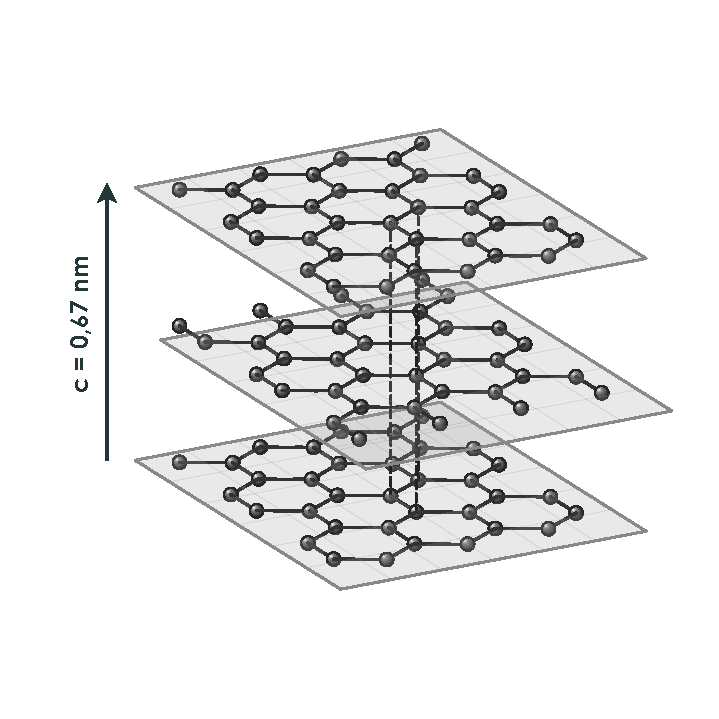
\includegraphics[width=0.45\linewidth]{FigurasSVG/UD3_Enlace_Quimico/pdf/UD3_51_grafito.pdf}
            \caption{Estructura atómica del grafito}
            \label{fig:grafito}
        \end{figure}

        \item La sílice (\ch{SiO2}) es un material muy duro formado por átomos de Si con una estructura tetraédrica en la que en cada extremo hay un átomo de oxígeno.
        La arena de la playa y el cuarzo son de sílice.
\end{enumerate}

\subsection{Propiedades de los compuestos covalentes}\label{subsec:propiedades-de-los-compuestos-covalentes}

A diferencia de las sustancias iónicas, las sustancias covalentes tendrán un tipo de propiedades según se enlacen como moléculas discretas o formen redes tridimensionales.

\begin{enumerate}[label=\numberballmDarkTeal]
        \item Los \textbf{sólidos covalentes} son sólidos de elevado \textbf{punto de fusión}, ya que, para fundirlos, hay que romper los enlaces covalentes que existen entre los átomos.
        \item Las \textbf{sustancias covalentes moleculares}  se pueden presentar a temperatura ambiente como sólidos, líquidos o gases dependiendo del tipo de fuerzas intermoleculares (se verán en el siguiente apartado) que presenten.
        En cualquier caso, estos compuestos presentan puntos de fusión y ebullición inferiores a los de los compuestos iónicos y metálicos.
        \item Las sustancias covalentes moleculares son \textbf{solubles en disolventes de polaridad similar}.
        Por ejemplo una sustancia polar como el etanol, se disuelve en disolventes polares como el agua o una sustancia apolar como las grasas se disuelven en disolventes apolares como el hexano.
        \item Las sustancias covalentes localizados  \textbf{no conducen la electricidad en ningún estado,} pero si son conductoras de la electricidad sustancias como el grafito que presentan una nube \(\bm{\pi}\) en la que puede existir la movilidad de los electrones.
        \item Las sustancias covalentes son \textbf{blandas y elásticas}.
        \item Los \textbf{sólidos covalentes} son \textbf{duros} y \textbf{frágiles}
\end{enumerate}


\section{Fuerzas intermoleculares}\label{sec:fuerzas-intermoleculares}

\begin{center}
    \begin{definicion}[width=0.9\textwidth]{Fuerzas intermoleculares}
        Son aquellas que se producen entre las distintas moléculas y, por tanto, no implica un enlace como tal
    \end{definicion}
\end{center}


Las fuerzas intermoleculares serán las que determine finalmente el \textbf{estado de agregación} y los \textbf{puntos de fusión y ebullición} de ese compuesto.
Además, estas fuerzas disminuyen al aumentar la distancia entre las moléculas por lo que es obvio decir que estas fuerzas son menos importantes o prácticamente irrelevantes en los gases, siendo relevantes en los sólidos y los líquidos.

Tenemos principalmente dos tipos de fuerzas:
\begin{enumerate}[label=\numberballmDarkTeal]
        \item \negsubro{Enlaces de hidrógeno}.
        Es un tipo de interacción \textbf{especial} que se da siempre entre un átomo de hidrógeno (\ch{H}) y un átomo electronegativo que suele ser el flúor (\ch{F}), oxígeno (\ch{O}) o nitrógeno (\ch{N}).

        La aparición de una carga parcial positiva ($\delta +$) en el hidrógeno y una carga parcial negativa ($\delta -$) en el átomo de \ch{F}, \ch{N} ó \ch{O} origina una atracción electrostática entre los átomos de una molécula de hidrógeno y los átomos más electronegativos de otra molécula.
        \begin{figure}[H]
            \centering
            % [FIGURA ORIGINAL] \includegraphics[scale=0.4]{images/imagesUD3EnlaceQuimico/UD3_Teoria/puentes_hidrogeno}
            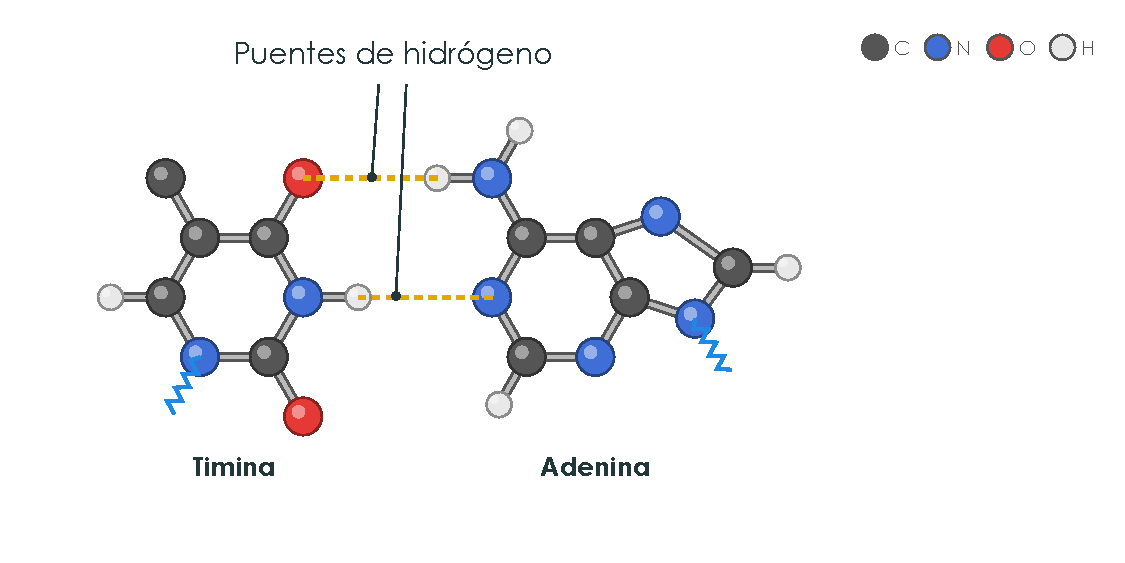
\includegraphics[width=0.6\linewidth]{FigurasSVG/UD3_Enlace_Quimico/pdf/UD3_52_puentes_hidrogeno_ADN.pdf}
            % [FIGURA ORIGINAL] \includegraphics[scale=0.3]{images/imagesUD3EnlaceQuimico/UD3_Teoria/puentes_hidrogeno_b}
            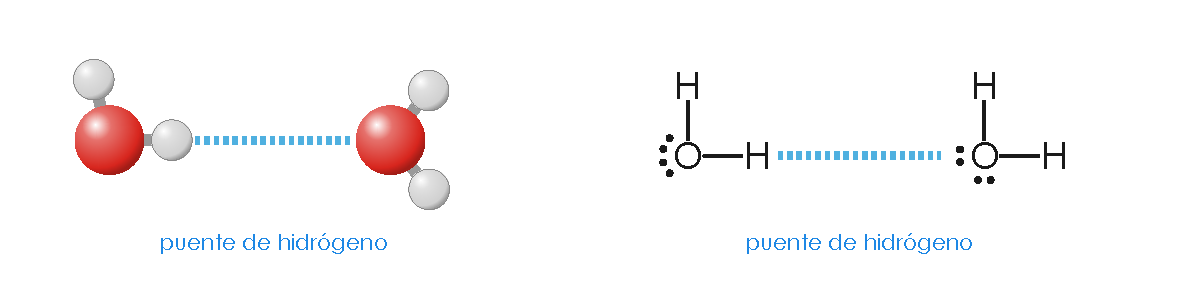
\includegraphics[width=0.6\linewidth]{FigurasSVG/UD3_Enlace_Quimico/pdf/UD3_53_puentes_hidrogeno_agua.pdf}
            \caption{Puentes de hidrógeno en la molécula de \ch{H2O}}\label{fig:puentes-de-hidrogeno}
        \end{figure}
        \begin{figure}[H]
            \centering
            % [FIGURA ORIGINAL] \includegraphics[scale=0.4]{images/imagesUD3EnlaceQuimico/UD3_Teoria/puentes_hidrogeno_c}
            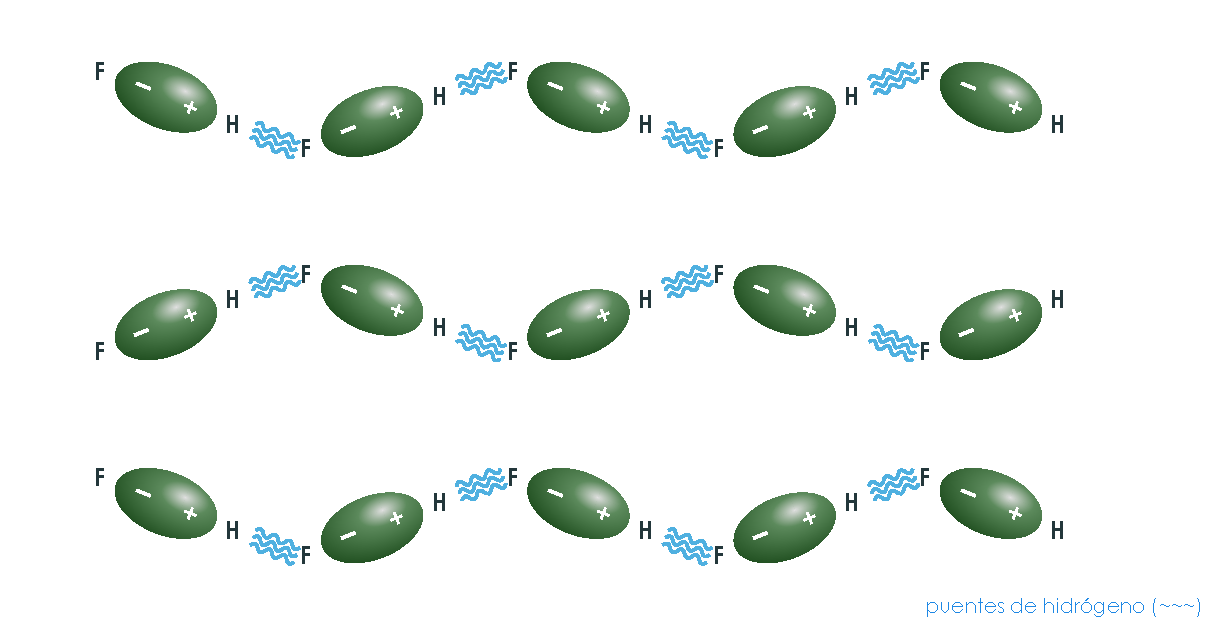
\includegraphics[width=0.6\linewidth]{FigurasSVG/UD3_Enlace_Quimico/pdf/UD3_54_puentes_hidrogeno_HF.pdf}
            \caption{Puentes de hidrógeno en la molécula de \ch{HF}}
            \label{fig:puentesdehidrogeno}
        \end{figure}
        \item \negsubro{Fuerzas de Van der Walls}
        \begin{enumerate}[label=\letraminuscula]
            \item \negrita{Fuerzas de London o dispersión}.
            Se da en moléculas \textbf{apolares}.
            La interacción se produce porque debido a las fluctuaciones de los electrones en la molécula se producen pequeños dipolos.
            \begin{figure}[H]
                \centering
                % [FIGURA ORIGINAL] \includegraphics[scale=0.5]{images/imagesUD3EnlaceQuimico/UD3_Teoria/fuerzaslondon}
                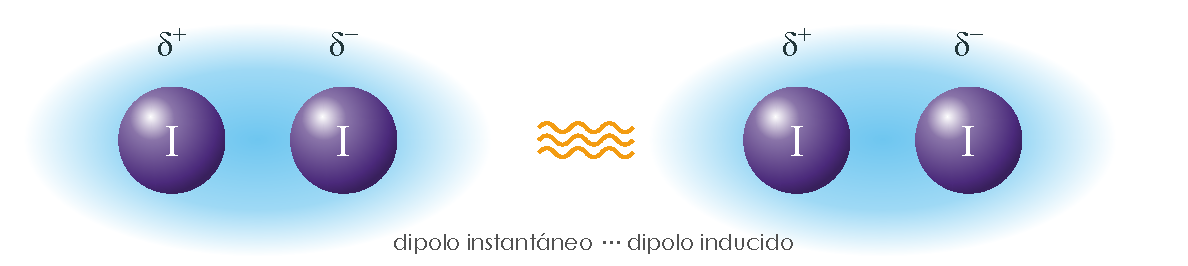
\includegraphics[width=0.6\linewidth]{FigurasSVG/UD3_Enlace_Quimico/pdf/UD3_55_fuerzas_london.pdf}
                \caption{Fuerzas de London en la molécula de \ch{F2}}
                \label{fig:fuerzasdelondon}
            \end{figure}
            \item \negrita{Fuerzas dipolo--dipolo}.
            Se produce entre moléculas \textbf{covalentes polares}.
            \begin{figure}[H]
                \centering
                % [FIGURA ORIGINAL] \includegraphics[scale=0.5]{images/imagesUD3EnlaceQuimico/UD3_Teoria/dipolodipolo}
                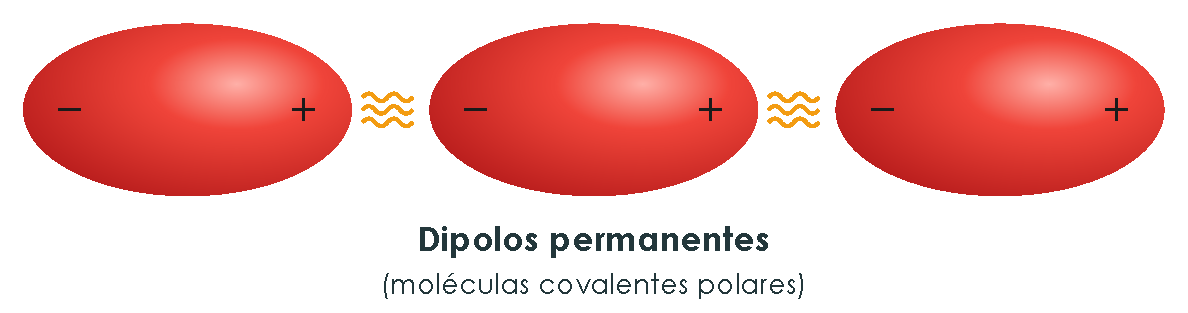
\includegraphics[width=0.6\linewidth]{FigurasSVG/UD3_Enlace_Quimico/pdf/UD3_56_dipolo_dipolo.pdf}
                \caption{Fuerzas dipolo--dipolo en la molécula de \ch{H2S}}
                \label{fig:fuerzasdipolodipolo}
            \end{figure}
            \item \negrita{Fuerzas dipolo--dipolo inducido}.
            Estas fuerzas aparece cuando mezclamos moléculas \textbf{polares} con \textbf{apolares}, las moléculas polares ya tienen un dipolo y estas inducen la generación de un dipolo en la moléculas apolares (dipolo inducido).
            \begin{figure}[H]
                \centering
                % [FIGURA ORIGINAL] \includegraphics[scale=0.5]{images/imagesUD3EnlaceQuimico/UD3_Teoria/dipolodipoloinducido}
                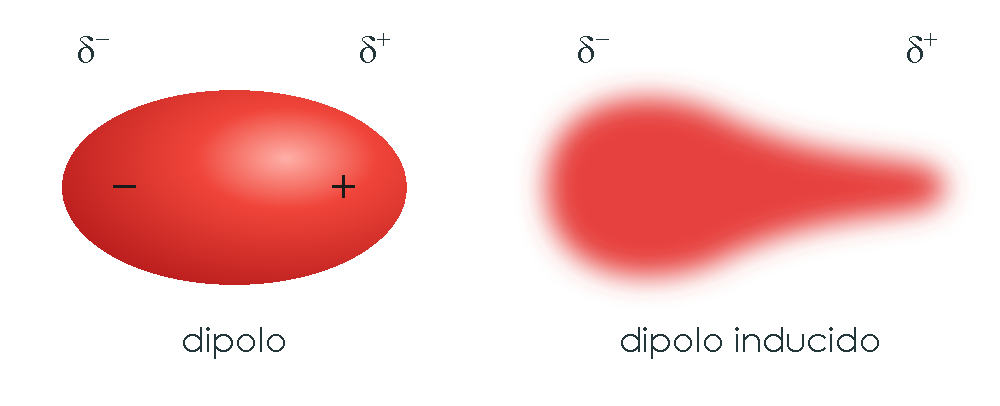
\includegraphics[width=0.55\linewidth]{FigurasSVG/UD3_Enlace_Quimico/pdf/UD3_57_dipolo_dipolo_inducido.pdf}
                \caption{Fuerzas dipolo--dipolo inducido}
                \label{fig:dipolodipoloinducido}
            \end{figure}
        \end{enumerate}
\end{enumerate}

\subsection{Fortaleza de las interacciones intermoleculares}\label{subsec:fortaleza-de-las-interacciones-intermoleculares}

No todos los enlaces intermoleculares presentan la misma fortaleza, el orden creciente en la fortaleza de las fuerzas intermoleculares es:

\caja{Enlaces de hidrógeno $>$ Fuerzas dipolo-dipolo $>$ Fuerzas dipolo-dipolo inducido $>$ Fuerzas de London }


\section{Enlace metálico}\label{sec:enlace-metalico}

Los metales constituyen el 80\% de los elementos químicos.
Las teorías para explicar el enlace metálico deben por tanto justificar las distintas propiedades de los metales.
Podemos destacar dos teorías:

\begin{enumerate}[label=\numberballmDarkTeal]
        \item \negsubro{Modelo de la nube electrónica: modelo de Drude}.
        Los cationes metálicos forman una red cristalina en cuyo interior hay una \azuln{nube de electrones} de valencia que se mueven libremente actuando también como unión de los iones positivos.
        La atracción electrostática entre los electrones y cationes mantiene fuertemente unidos a todos los átomos del metal.
        \begin{figure}[H]
            \centering
            % [FIGURA ORIGINAL] \includegraphics[scale=0.5]{images/imagesUD3EnlaceQuimico/UD3_Teoria/enlacemetalico_nubeelectronica}
            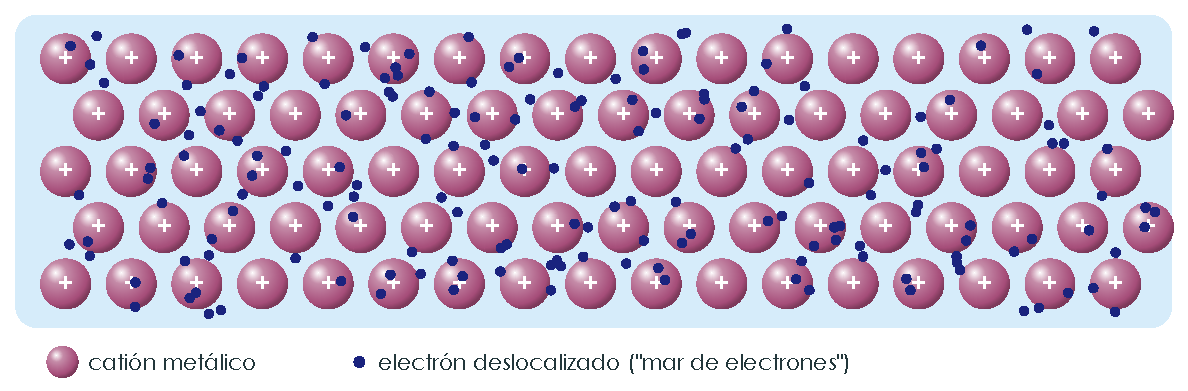
\includegraphics[width=0.8\linewidth]{FigurasSVG/UD3_Enlace_Quimico/pdf/UD3_58_enlace_metalico.pdf}
            \caption{Modelo de la nube electrónica del enlace metálico}
            \label{fig:modelonubeelectronica}
        \end{figure}
        Este modelo explica algunas propiedades de los metales como la conductividad eléctrica, brillo metálico etc., pero no otras como el comportamiento de los semiconductores.
        \item \negsubro{Teoría de bandas}.
        Es un modelo que se basa en el modelo cuántico de la teoría de los OOMM. A medida que aumentamos el número de orbitales atómicos, aumentamos el número de orbitales moleculares y si es lo suficientemente grande los niveles energéticos se suceden dando lugar a \azuln{bandas de energía}.

        \xmybox{\negrita{Teoría de bandas para el \ch{Mg}}}. \ch{Mg} = \elconf{12}.
        El magnesio tiene dos electrones situados en el orbital $3s$, quedando los orbitales $3p$ vacíos.
        Si consideramos el metal como muchos átomos de magnesio juntos, podemos imaginar la aparición de bandas formadas por muchos orbitales superpuestos.

%        \begin{figure}[H]
%            \centering
%            \includegraphics[scale=.75]{images/imagesUD3EnlaceQuimico/UD3_Teoria/teoriadebandas}
%            \caption{Teoría de bandas}
%            \label{fig:teoria-de-bandas}
%        \end{figure}

        Una banda, correspondiente a la superposición de orbitales $3s$, estará llena de electrones y se llamará \azuln{banda de valencia} y otra banda compuesta por los orbitales $3p$ vacíos se denominará \azuln{banda de conducción}.


        Dichas bandas, en general están separadas por regiones de energía prohibidas llamadas \blueremark{gap} aunque en algunos casos se puede producir la superposición entre bandas con solapamiento energético.

        Con esta teoría se puede comprender fácilmente el comportamiento como \azuln{conductores}, \azuln{semiconductores}, \azuln{aislantes}.
        \begin{figure}[H]
            \centering
            % [FIGURA ORIGINAL] \includegraphics[scale=.5]{images/imagesUD3EnlaceQuimico/UD3_Teoria/teoriadebandas}
            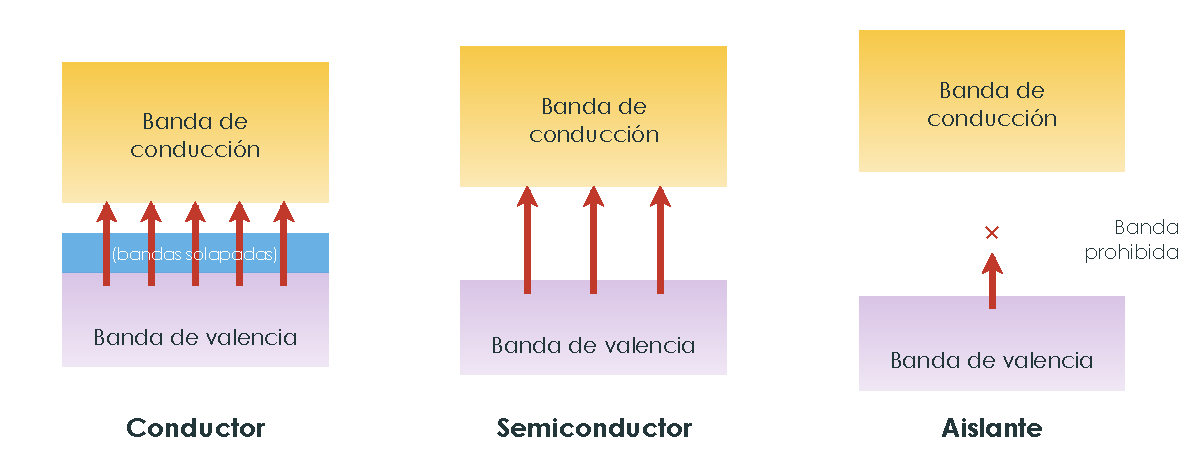
\includegraphics[width=0.75\linewidth]{FigurasSVG/UD3_Enlace_Quimico/pdf/UD3_59_teoria_bandas.pdf}
            \caption{Teoría de bandas}
            \label{fig:teoriadebandas}
        \end{figure}
        \begin{enumerate}[label=\numberballred]
            \item \negrita{Conductores}.
            Son aquellos en los que la banda de valencia y la banda de conducción presentan una diferencia energética muy pequeña o bien están solapando.
            \item \negrita{Semiconductores}.
            Son aquellos en los que la diferencia de la banda de valencia y la banda de conducción no es muy grande.
            \item \negrita{Aislantes}.
            Son aquellos en los que la diferencia de la banda de valencia y la banda de conducción es muy grande.
        \end{enumerate}
\end{enumerate}

\subsection{Propiedades del enlace metálico}\label{subsec:propiedades-del-enlace-metalico}
Las principales propiedades de los metales son:

\begin{enumerate}[label=\numberballmDarkTeal]
        \item Los compuestos metálicos presentan un \textbf{brillo metálico}.
        \item Suelen ser \textbf{sólidos} a excepción del mercurio \ch{Hg}.
        \item Presentan una \textbf{elevada densidad}.
        \item Son \textbf{dúctiles} es decir se deforman en hilos y también son \textbf{maleables} es decir capacidad para deformarse en láminas.
        \item Son buenos \textbf{conductores de la electricidad y el calor}.
        \item Son \textbf{insolubles}.
\end{enumerate}

% \begin{enumerate}[label=\numberballred]
%     \item \negrita{Brillo}. Los compuestos metálicos tienen brillo.
%     \item \negrita{Estado de agregación}. Son sólidos con elevados puntos de ebullición y de fusión.
%     \item \negrita{Densidad}. Presentan una densidad elevada.
%     \item \negrita{Propiedades mecánicas}. Son dúctiles (al deformarse se forman hilos) y maleables (capacidad de deformarse en láminas).
%     \item \negrita{Conductividad eléctrica y térmica}. Son buenos conductores de la electricidad y el calor.
%     \item \negrita{Solubilidad}. Son insolubles en disolventes moléculas.
% \end{enumerate}

